\documentclass[10pt]{article}

% Be sure to use PDF Latex
\pdfoutput=1

% links
\usepackage[bookmarks,bookmarksdepth=2, colorlinks=true, linkcolor=blue,citecolor=red, urlcolor=blue]{hyperref}


\usepackage{fullpage}

\usepackage[latin1]{inputenc}
\usepackage{mystyle}
\usepackage{wrapfig}
\usepackage{notations_ot} % for OT chapter
\usepackage{tikz}

\newcommand{\dims}{d}


\graphicspath{{./figures/}}


\newcommand{\myauthor}[3]{#1\protect\footnote{#2, \protect\url{#3}}}


\title{Course notes on\\ Computational Optimal Transport} 

\author{%
\begin{tabular}{c}
	Gabriel Peyr{\'e} \\ CNRS \& DMA \\
	 \'Ecole Normale Sup\'erieure \\
	 \url{gabriel.peyre@ens.fr}\\
	 \url{https://mathematical-tours.github.io}\\
	 \url{www.numerical-tours.com}
\end{tabular}
}


\date{\today}

%%

\begin{document}

\maketitle

\begin{abstract}
These course notes present the foundational mathematics concepts relevant to computational optimal transport. They delve into various formulations and techniques, starting with Monge's formulation, illustrated through applications to one-dimensional optimal transport and distributions involving Gaussians. The notes then explore Kantorovich's formulation, a more general approach that addresses limitations in Monge's method and applies to a wider range of problems.
%
Additionally, the course covers the concept of the Wasserstein distance, a key metric in optimal transport theory that quantifies the cost of transporting one distribution to another.
%
The notes also introduce entropic regularization, an important technique used to smooth optimization problems and make them more tractable computationally. This approach facilitates the numerical solution of optimal transport problems by adding an entropy term to the objective function, leading to faster and more stable algorithms.
%
Finally, the dual formulation of optimal transport problems is presented. This perspective allows for deriving alternative algorithms and insights into the structure of optimal transport solutions. By exploring the dual problem, students can understand the relationships between different formulations and how they can be exploited to solve transport problems more efficiently.
%
Overall, these course notes provide a comprehensive introduction to the mathematics of computational optimal transport, offering insights into both theoretical foundations and practical applications.
\end{abstract}

% \tableofcontents

% !TEX root = ../CourseOT.tex

%%%%%%%%%%%%%%%%%%%%%%%%%%%%%%%%%%%%%%%%%%%%%%%%%%%%%%%%%%%%%%%%%%%%%%%%%%%
%%%%%%%%%%%%%%%%%%%%%%%%%%%%%%%%%%%%%%%%%%%%%%%%%%%%%%%%%%%%%%%%%%%%%%%%%%%
%%%%%%%%%%%%%%%%%%%%%%%%%%%%%%%%%%%%%%%%%%%%%%%%%%%%%%%%%%%%%%%%%%%%%%%%%%%
\section{Optimal Matching between Point Clouds}

%%%%%%%%%%%%%%%%%%%%%%%%%%%%%%%%%%%%%%%%%%%%%%%%%%%%%%%%%%%%%%%%%%%%%%%%%%%
\subsection{Monge Problem for Discrete Points}
\label{sec-monge-pbm}

%%%%%%%
\paragraph{Matching Problem}

Given a cost matrix $(\C_{i,j})_{i \in \range{n}, j \in \range{m}}$ and assuming $n=m$, the optimal assignment problem aims to find a bijection $\sigma$ within the set $\Perm(n)$ of permutations of $n$ elements that solves
\eql{\label{eq-optimal-assignment}
	\umin{\sigma \in \Perm(n)} \frac{1}{n}\sum_{i=1}^n \C_{i,\sigma(i)}.
}
One could naively evaluate the cost function above using all permutations in the set $\Perm(n)$. However, this set has size $n!$, which becomes enormous even for small values of $n$.
%
In general, the optimal $\sigma$ is not unique.


\paragraph{1D Case}

If the cost is of the form $\C_{i,j}=h(x_i-y_j)$, where $h: \RR \rightarrow \RR^+$ is convex (for example, $\C_{i,j}=|x_i-y_j|^p$ for $p \geq 1$), it follows that an optimal $\sigma$ necessarily defines an increasing map $x_i \mapsto y_{\sigma(i)}$, i.e.,
\eq{
	\forall (i,i'), \quad (x_i-x_{i'})(y_{\sigma(i)}-y_{\sigma(i')}) \geq 0.
}
Indeed, if this property is violated, i.e., there exists $(i,i')$ such that $(x_i-x_{i'})(y_{\sigma(i)}-y_{\sigma(i')}) < 0$, then one can define a permutation $\tilde{\sigma}$ by swapping the match, i.e., $\tilde{\sigma}(i)=\sigma(i')$ and $\tilde{\sigma}(i')=\sigma(i)$, yielding a better cost
\eq{
	\sum_i h(x_{i}-y_{\tilde{\sigma}(i)}) \leq \sum_i h(x_{i}-y_{\sigma(i)}),  
}
because
\eq{
	h(x_{i}-y_{\tilde\sigma(i')}) + h(x_{i'}-y_{\tilde\sigma(i)}) 
	\leq
	h(x_{i}-y_{\sigma(i)}) + h(x_{i'}-y_{\sigma(i')}).  
}
Therefore, the algorithm to compute an optimal transport is to sort the points, i.e., find some pair of permutations $\sigma_X, \sigma_Y$ such that
\eq{
	x_{\sigma_X(1)} \leq x_{\sigma_X(2)} \leq \ldots
	\qandq
	y_{\sigma_Y(1)} \leq y_{\sigma_Y(2)} \leq \ldots
}
and then an optimal match is mapping $x_{\sigma_X(k)} \mapsto y_{\sigma_Y(k)}$, i.e., an optimal transport is $\sigma = \sigma_Y \circ \sigma_X^{-1}$. The total computational cost is thus $O(n\log(n))$, using, for instance, the quicksort algorithm.
%
Note that if $\phi : \RR \rightarrow \RR$ is an increasing map, one can apply this technique to costs of the form $h(|\phi(x)-\phi(y)|)$ with a change of variable.
%
A typical application is the grayscale histogram equalization of the luminance of images.

Note that if $h$ is strictly convex, then all optimal assignement are increasing, so if the points are all distincts, there is a unique such increasing map. But if $h$ is not strictly convex, for instance $c(x,y)=|x-y|$ then there exists non increasing optimal assignement, for instance in the book shifting problem, with overlapping uniform distribution (the mass at the intesection can stay at the same place).

This efficient strategy to compute the OT in 1-D does not extend to higher dimensions. In 2-D, if the cost is $c(x,y) = \norm{x-y}$, then, as already noted by Monge, trajectories cannot cross, this is a consequence of the parallelogram inequality. However, this is not enough to uniquely determine an optimal matching. 

Note that if $h$ is concave instead of being convex, then the behavior is entirely different, and the optimal match tends to exchange the positions. In this case, there exists an $O(n^2)$ algorithm.


%%%%%%%%%%%%%%%%%%%%%%%%%%%%%%%%%%%%%%%%%%%%%%%%%%%%%%%%%%%%%%%%%%%%%%%%%%%
\subsection{Matching Algorithms}

Efficient algorithms exist to solve the optimal matching problem. The most well-known are the Hungarian and the auction algorithm, which run in $O(n^3)$ operations. Their derivation and analysis, however, are greatly simplified by introducing the Kantorovich relaxation and its associated dual problem.
%
A typical application of these methods is equalizing the color palette between images, corresponding to a 3-D optimal transport.

% !TEX root = ../CourseOT.tex

%%%%%%%%%%%%%%%%%%%%%%%%%%%%%%%%%%%%%%%%%%%%%%%%%%%%%%%%%%%%%%%%%%%%%%%%%%%
%%%%%%%%%%%%%%%%%%%%%%%%%%%%%%%%%%%%%%%%%%%%%%%%%%%%%%%%%%%%%%%%%%%%%%%%%%%
%%%%%%%%%%%%%%%%%%%%%%%%%%%%%%%%%%%%%%%%%%%%%%%%%%%%%%%%%%%%%%%%%%%%%%%%%%%
\section{Monge Problem between Measures}

The presentation of the previous section could only handle two sets with the same number of points. To relax this to more general setting, one needs to consider probability distribution, so that the points are now weighted by some mass. 

%%%%%%%%%%%%%%%%%%%%%%%%%%%%%%%%%%%%%%%%%%%%%%%%%%%%%%%%%%%%%%%%%%%%%%%%%%%
\subsection{Measures}


%%%
\paragraph{Histograms}

We will interchangeably the term histogram or probability vector for any element $\a \in \simplex_n$ that belongs to the probability simplex
\eq{
	\simplex_n \eqdef \enscond{\a \in \RR_+^n}{ \sum_{i=1}^n \a_i = 1 }.
}


%%%
\paragraph{Discrete measure, empirical measure}

A discrete measure with weights $\a$ and locations $x_1,\dots,x_n\in\X$ reads
\eql{\label{eq-discr-meas}
	\al = \sum_{i=1}^n \a_i \de_{x_i}
}
where $\de_x$ is the Dirac at position $x$, intuitively a unit of mass which is infinitely concentrated at location $x$. Such a measure describes a probability measure if, additionally, $\a\in\simplex_n$, and more generally a positive measure if each of the ``weights'' described in vector $\a$ is positive itself. 
%
An ``empirical'' probability distribution is uniform on a point cloud, i.e. $\a=\frac{1}{n}\sum_i \de_{x_i}$. 
%
In practice, in many applications, it is useful to be able to manipulate both the positions $x_i$ (``Lagrangian'' discretization) and the weights $\a_i$ (``Eulerian'' discretization). Lagrangian modification is usually more powerful (because it leads to adaptive discretization) but it breaks the convexity of most problems. 


%%%%
\paragraph{General measures}

We consider Borel measures $\al \in \Mm(\X)$ on a metric space $(\Xx,d)$, i.e. one can compute $\al(A)$ for any Borel set $A$ (which can be obtained by applying countable union, countable intersection, and relative complement to open sets). The measure should be finite, i.e. have a finite value on compact sets.
%
A Dirac measure $\de_x$ is then defined as $\de_x(A)=1$ is $x \in A$ and $0$ otherwise, and this extends by linearity for discrete measures of the form~\eqref{eq-discr-meas} as
\eq{
	\al(A) = \sum_{x_i \in A} \a_i  
}
%
We denote $\Mm_+(\X)$ the subset of all positive measures on $\X$, i.e. $\al(A) \geq 0$ (and $\al(\X)<+\infty$ for the measure to be finite). The set of probability measures is denoted $\Mm_+^1(\X)$, which means that any $\al \in \Mm_+^1(\X)$ is positive, and that $\al(\X)=1$. 


%%%%
\paragraph{Radon measures}

Using Lebesgue integration, a Borel measure can be used to compute the integral of measurable functions (i.e. such that level sets $\enscond{x}{f(x) < t}$ are Borel sets), and we denote this pairing as
\eq{
	\dotp{f}{\al} \eqdef \int f(x) \d\al(x).
}
Integration of such a measurable $f$ against a discrete measure $\al$ computes a sum
\eq{ 
	\int_\X f(x) \d\al(x) = \sum_{i=1}^n \a_i f(x_i).
}

 
This can be in particular applied to the subspace of continuous functions which are measurable.
%
Integration against a finite measure on a compact space thus defines a continuous linear form $f \mapsto \int f \d\al$ on the Banach space of continuous functions $(\Cc(\Xx),\norm{\cdot}_\infty)$, indeed $|\int f \d\al| \leq \norm{f}_\infty |\al(\X)|$. 
%
On compact spaces, the converse is true, namely that any continuous linear form $\ell : f \mapsto \ell(f)$ on $(\Cc(\Xx),\norm{\cdot}_\infty)$ is represented as an integral against a measure $\ell(f)=\int f \d \al$. This is the  Riesz-Markov-Kakutani representation theorem, which is often stated that Borel measures can be identified to Radon measures.
%
Radon measures are thus in some sense ``less regular'' than functions, but more regular than distributions (which are dual to smooth functions). For instance, the derivative of a Dirac is not a measure.
%
This duality pairing $\dotp{f}{\al}$ between continuous function and measures will be crucial to developing duality theory for the convex optimization problem we will consider later. 

The associated norm, which is the norm of the linear form $\ell$, is the so-called total variation norm
\eq{
	\norm{\al}_{\mathrm{TV}} = \norm{\ell}_{\Cc(\Xx)\rightarrow \RR} = \usup{f \in \Cc(\X)} \enscond{\dotp{f}{\al}}{ \norm{f}_\infty \leq 1 }.
}
(note that one can remove the $|\cdot|$ on the right-hand side, and such a quantity is often called a ``dual norm'').
%
One can show that this TV norm is the total mass of the absolute value measure $|\al|$.
%
The space $(\Mm(\Xx),\norm{\cdot}_{TV})$ is a Banach space, which is the dual of $(\Cc(\Xx),\norm{\cdot}_\infty)$. 

Recall that the absolute value of a measure is defined as 
\eq{
	|\al|(A) = \usup{A=\cup_i B_i} \sum_i |\al(B_i)|
}
so that for instance if $\al=\sum_i \a_i \de_{x_i}$, $|\al|=\sum_i |\a_i| \de_{x_i}$ and if $\d\al(x) = \rho \d x$ for a positif reference measure $\d x$, then $\d|\al|(x) = |\rho(x)| \d x$. 



%%%%%
\paragraph{Relative densities}

%TODO : ref measures
A measure $\al$ which is a weighting of another reference one $\d x$ is said to have a density, which is denoted $\d\al(x)=\density{\al}(x)\d x$  (on $\RR^d$ $\d x$ is often the Lebesgue measure), often also denoted $\density{\al} = \frac{\d\al}{\d x}$, which means that 
\eq{
	\foralls h \in \Cc(\RR^\dims), \quad
	\int_{\RR^\dims} h(x) \d\al(x) =  \int_{\RR^\dims} h(x) \density{\al}(x) \d x.
}

%%%%%
\paragraph{Probabilistic interpretation}

Radon probability measures can also be viewed as representing the distributions of random variables. A random variable $X$ on $\X$ is actually a map $X : \Om \rightarrow \X$ from some abstract (often un-specified) probabized space $(\Om,\PP)$, and its distribution is the Radon measure $\al \in \Mm_+^1(\X)$ such that $\PP(X \in A) = \al(A)=\int_A \d\al(x)$.


%%%%%%%%%%%%%%%%%%%%%%%%%%%%%%%%%%%%%%%%%%%%%%%%%%%%%%%%%%%%%%%%%%%%%%%%%%%
\subsection{Push Forward}
  
  
For some continuous map $\T : \X \rightarrow \Y$, we define the pushforward operator $\T_\sharp : \Mm(\X) \rightarrow \Mm(\Y)$. 
%
For a Dirac mass, one has $\T_\sharp \de_{x} = \de_{\T(x)}$, and this formula is extended to arbitrary measure by linearity. In some sense, moving from $\T$ to $\T_\sharp$ is a way to linearize any map at the prize of moving from a (possibly) finite dimensional space $\Xx$ to the infinite dimensional space $\Mm(\Xx)$, and this idea is central to many convex relaxation method, most notably Lasserre's relaxation.
%
For discrete measures~\eqref{eq-discr-meas}, the pushforward operation consists simply in moving the positions of all the points in the support of the measure
\eq{
	\T_{\sharp} \al \eqdef \sum_i \a_i \de_{\T(x_i)}.
}
For more general measures, for instance for those with a density, the notion of push-forward plays a fundamental to describe spatial modifications of probability measures. The formal definition reads as follow.

\begin{defn}[Push-forward]\label{defn-pushfwd}
For $\T : \X \rightarrow \Y$, the push forward measure $\be = \T_\sharp \al \in \Mm(\Y)$ of some $\al \in \Mm(\X)$ satisfies
\eql{\label{eq-push-fwd}
	\foralls h \in \Cc(\Y), \quad \int_\Y h(y) \d \be(y) = \int_\X h(\T(x)) \d\al(x).
}
Equivalently, for any measurable set $B \subset \Y$, one has
\eql{\label{eq-equiv-pushfwd}
	\be(B) = \al( \enscond{x \in \X}{\T(x) \in B} ).
}
Note that $\T_\sharp$ preserves positivity and total mass, so that if $\al \in \Mm_+^1(\X)$ then $\T_\sharp \al \in \Mm_+^1(\Y)$. 
\end{defn}



%%%%%%%
\begin{rem}[Push-forward for densities]
Explicitly doing the change of variable $y=T(x)$, so that $\d y = |\det(T'(x))| \d x$ in formula~\eqref{eq-push-fwd} for measures with densities $(\density{\al},\density{\be})$ on $\RR^\dims$ (assuming $\T$ is smooth and a bijection), one has for all $h \in \Cc(\Yy)$
\begin{align*}
	\int_\Yy h(y)\rho_\be(y) \d y &= \int_\Yy h(y) \d \be(y) = \int_\Xx h(T(x)) \d \al(x) = \int_\Xx h(T(x)) \rho_\al(x) \d x \\
		&= \int_\Yy h(y) \rho_\al(T^{-1}y) \frac{\d y}{|\det(T'( T^{-1} y))|}, 
\end{align*}
which shows that 
\eq{
	\rho_\be(y) = \rho_\al(T^{-1}y) \frac{1}{|\det(T'( T^{-1} y))|}.
}
Since $T$ is a diffeomorphism, one obtains equivalently
\eql{\label{eq-pfwd-density}
	\density{\al}(x) = |\det(\T'(x))|  \density{\be}(\T(x))
}
where $\T'(x) \in \RR^{\dims \times \dims}$ is the Jacobian matrix of $T$ (the matrix formed by taking the gradient of each coordinate of $T$).
%
This implies, denoting $y=\T(x)$
\eq{
	|\det(\T'(x))| = \frac{ \density{\al}(x) }{ \density{\be}(y) }.
}
\end{rem}
%%%%%%%


\begin{rem}[Probabilistic interpretation]
A random variable $X$, equivalently, is the push-forward of $\PP$ by $X$, $\al=X_\sharp\PP$.
%
Applying another push-forward $\be = \T_\sharp\al$ for $\T : \X \rightarrow \Y$, following~\eqref{eq-push-fwd}, is equivalent to defining another random variable $Y=\T(X) : \om \in \Om \rightarrow \T(X(\om)) \in Y$, so that $\be$ is the distribution of $Y$.
%
Drawing a random sample $y$ from $Y$ is thus simply achieved by computing $y=\T(x)$ where $x$ is drawn from $X$. 
\end{rem}


%%%%%%%%%%%%%%%%%%%%%%%%%%%%%%%%%%%%%%%%%%%%%%%%%%%%%%%%%%%%%%%%%%%%%%%%%%%
\subsection{Monge's Formulation}


%%%%
\paragraph{Monge problem.}

Monge problem~\eqref{eq-optimal-assignment} is extended to the setting of two arbitrary probability measures $(\al,\be)$ on two spaces $(\X,\Y)$ as finding a map $\T : \X \rightarrow \Y$ that minimizes
\eql{\label{eq-monge-continuous}
	\uinf{\T} \enscond{ \int_{\X} \c(x,\T(x)) \d \al(x)  }{  \T_\sharp \al = \be }.
}
The constraint $\T_\sharp \al = \be$ means that $\T$ pushes forward the mass of $\al$ to $\be$, and makes use of the push-forward operator~\eqref{eq-push-fwd}. 

For empirical measures with the same number $n=m$ of points, one retrieves the optimal matching problem. Indeed, this corresponds to the setting of empirical measures $\al=\frac{1}{n}\sum_{i=1}^n \de_{x_i}$ and $\be=\frac{1}{n}\sum_{i=1}^n \de_{y_i}$. In this case, $\T_\sharp \al=\be$ necessarily implies that $\si$ is subjective, hence it is one-to-one, and it induces a permutation $\sigma$ on the support, $\T : x_i \mapsto x_{\si(i)}$, so that 
\eq{
	\int_{\X} \c(x,\T(x)) \d \al(x) = \sum_i c(x_i,x_{\si(i)}).
}

In general, an optimal map $T$ solving~\eqref{eq-monge-continuous} might fail to exist. The constraint set $\T_\sharp \al = \be$, which is the case for instance if $\al=\de_x$ and $\be$ is not a single Dirac. 

Note that even if the constraint set is not empty the infimum might not be reached, the most celebrated example being the case of $\al$ being distributed uniformly on a single segment and $\be$ being distributed on two segments on the two sides.

\paragraph{Semi-discrete setting.}

It is also not a symmetric problem in $\alpha$ and $\beta$. For instance, this problem makes sense if $\alpha$ has a density with respect to Lebesgue and $\beta$ is discrete. It is a semi-discrete problem, which can be understood as an optimal quantization problem. 
%
Indeed, for instance on $\X=\Y=\RR^d$, one can consider a setting where $\alpha$ has a density with respect to Lebesgues and $\beta = \sum_j b_j \delta_{y_j}$ is discrete, supported on $\{y_1,\ldots,y_m\}$. In this case, a  map $\T$ so that $\T_\sharp \alpha=\beta$ defines a segemtation of the space into $m$ cells $C_j := \T^{-1}(y_j)$, so that $\alpha(C_j)=b_j$. This is often reffered to as the semi-discrete setting. 
%
If one exchanges the role of $\alpha$ and $\beta$ (so that $\alpha$ is discrete) then there is not any valid $\T$.  
Indeed, it is not possible to push-forward a discrete measure to a measure with density, so that the constraint set of the Monge problem is empty. 



%%%%
\paragraph{Monge distance.}

In the special case $c(x,y)=d^p(x,y)$ where $d$ is a distance, we denote 
\eql{\label{eq-monge-distance}
	\tilde\Wass_p^p(\al,\be) \eqdef 
		\uinf{\T} \enscond{ \Ee_\al(T) \eqdef \int_{\X} d(x,\T(x))^p \d \al(x)  }{  \T_\sharp \al = \be }.
}
If the constraint set is empty, then we set $\tilde \Wass_p^p(\al,\be) = +\infty$.
%
The following proposition shows that quantity defines a (pseudo-) distance (because it is not symmetric).

\begin{prop}
	$\tilde \Wass$ is a non-symmetric distance.
\end{prop}
\begin{proof}
	If $\tilde \Wass_p^p(\al,\be)=0$ then necessarily the optimal map is $\Id$ on the support of $\al$ and $\be=\al$.
	%
	Let us prove that $\tilde \Wass_p(\al,\be) \leq \tilde \Wass_p(\al,\ga)+\tilde \Wass_p(\ga,\be)$.
	If $\tilde \Wass_p(\al,\be)=+\infty$, then either $\tilde \Wass_p(\al,\ga)=+\infty$ or $\tilde \Wass_p(\ga,\be)=+\infty$, because otherwise we consider two maps $(S,T)$ such that $S_\sharp \al=\ga$ and $T_\sharp \ga=\be$ and then $(T \circ S)_\sharp \al = \be$ so that 
	$\tilde \Wass_p^p(\al,\be) \leq \Ee_\al(S \circ T) < +\infty$.
	%
	So necessarily $\tilde \Wass_p^p(\al,\be)<+\infty$ and we can restrict our attention to the cases 
	where $\tilde \Wass_p^p(\al,\ga)<+\infty$ and $\tilde \Wass_p^p(\ga,\be)<+\infty$ because otherwise the inequality is trivial.
	%
	For any $\epsilon>0$, we consider $\epsilon$-minimizer $S_\sharp \al=\ga$ and $T_\sharp \ga=\be$ such that
	\eq{
		E_\al(S)^{\frac{1}{p}} \leq \tilde \Wass_p(\al,\ga)+\epsilon
		\qandq
		E_\ga(T)^{\frac{1}{p}} \leq \tilde \Wass_p(\ga,\be)+\epsilon.
	}
	%
	Now we have that $(T \circ S)_\sharp \al=\ga$, so that 
	one has, using sub-optimality of this map and the triangular inequality 
	\eq{
		\bar\Wass_p(\al,\ga) \leq \int d(x,T(S(x)))^p \d\al(x)^{\frac{1}{p}}
			\leq
			\int (d(x,S(x)) + d(S(x),T(S(x))))^p \d\al(x)^{\frac{1}{p}}	.		
	}
	The using Minkowski inequality for the $L^p$ spaces with measure $\al$ 
	\eq{
		\norm{f+g}_{L^p(\al)} \leq \norm{f}_{L^p(\al)} + \norm{g}_{L^p(\al)}
	}
	and with $f(x) \triangleq d(x,S(x))$ and $g(x) \triangleq d(S(x),T(S(x)))$
	one has
	\eq{
		\bar\Wass_p(\al,\ga) \leq
			\int d(x,S(x))^p \d\al(x)^{\frac{1}{p}}	
			+ 		
			\int d(S(x),T(S(x)))^p \d\al(x)^{\frac{1}{p}}	
			= 
			\int d(x,S(x))^p \d\al(x)^{\frac{1}{p}}	
			+ 		
			\int d(y,T(y))^p \d\be(y)^{\frac{1}{p}}	
	}
	$$
		\leq \Wass_p(\al,\be) + \Wass_p(\be,\ga) + 2 \epsilon.
	$$
	Letting $\epsilon \rightarrow 0$ gives the result. 
\end{proof}

This quantity $\tilde\Wass_p$ is problematic because it can have the value $+\infty$. It is the purpose of the Kantorovitch formulation exposed below to remedy this issue, to define a symmetric and well-behaved distance $\Wass_p$.

%%%%%%%%%%%%%%%%%%%%%%%%%%%%%%%%%%%%%%%%%%%%%%%%%%%%%%%%%%%%%%%%%%%%%%%%%%%
\subsection{Existence and Uniqueness of the Monge Map}

%%%%
\paragraph{Brenier's theorem.}

The following celebrated theorem of~\cite{Brenier91} ensures that in $\RR^\dims$ for $p=2$, if at least one of the two input measures has a density, then Monge's problem has a unique solution, and it gives a precise description of the structure of this solution.

\begin{thm}[Brenier]\label{thm-brenier}
	In the case $\X=\Y=\RR^\dims$ and $c(x,y)=\norm{x-y}^2$, if $\al$ has a density with respect to the Lebesgue measure, then there exists a unique optimal Monge map $\T$. This map is characterized by being the unique gradient of a convex function $\T=\nabla \phi$ such that $(\nabla \phi)_\sharp \al = \be$. 
\end{thm}

Its proof requires to study of the relaxed Kantorovitch problems and its dual, so we defer it to later (Section~\ref{sec-c-transfo}). 

Brenier's theorem, stating that an optimal transport map must be the gradient of a convex function, should be examined under the light that a convex function is a natural generalization of the notion of increasing functions in dimension more than one. 
%
For instance, the gradient of a convex function is a monotone gradient field in the sense
\eq{
	\foralls (x,x') \in \RR^d \times \RR^d, \quad 
	\dotp{\nabla\phi(x)-\nabla\phi(x')}{x-x'} \geq 0.
}
Note however that in dimensions larger than 1, not all monotone fields are gradients of convex functions. For instance, a small enough rotation is monotone but can never be an optimal transport because a gradient field $Ax$ defined by a linear map $A$ is necessarily obtained by a symmetric matrix $A$. Indeed, such a linear field must be associated with a quadratic form $\phi(x)=\dotp{Bx}{x}/2$
and hence $A=\nabla \phi = (B+B^\top)/2$.
%
Optimal transport can thus play an important role in defining quantile functions in arbitrary dimensions, which in turn is useful for applications to quantile regression problems~\cite{carlier2016vector}.
 
Note also that this theorem can be extended in many directions.  
% 
The condition that $\al$ has a density can be weakened to the condition that it does not give mass to ``small sets'' having Hausdorff dimension smaller than $\dims-1$ (e.g. hypersurfaces). 
%
One can also consider costs of the form $\c(x,y)=h(x-y)$ where $h$ is a strictly convex smooth function, for instance, $c(x,y)=\norm{x-y}^p$ with $1<p<+\infty$. 

Note that Brenier's theorem provides existence and uniqueness, but in general, the map $\T$ can be very irregular. 
%
Indeed, $\phi$ is in general non-smooth, but it is convex and Lipschitz so that $\nabla \phi$ is well defined $\al$-almost everywhere. Ensuring $\T$ to be smooth requires the target $\be$ to be regular, and more precisely its support must be convex.

If $\al$ does not have a density, then $\T$ might fail to exist and it should be replaced by a set-valued function included in $\partial\phi$ which is now the sub-differential of a convex function, which might have singularity on a non-zero measure set. This means that $\T$ can ``split'' the mass by mapping to several locations  $T(x) \subset \partial\phi$. The condition that $T(x) \subset \partial\phi(x)$ and $\T_\sharp \al=\be$ implies that the multi-map $\T$ defines a solution of Kantorovitch problem that will be studied later. 


%%%%%%%
\paragraph{Monge-Amp\`ere equation.}

For measures with densities, using~\eqref{eq-pfwd-density}, one obtains that $\phi$ is the unique (up to the addition of a constant) convex function which solves the following Monge-Amp\`ere-type equation
\eql{\label{eq-monge-ampere}
	\det(\partial^2\phi(x))  \density{\be}(\nabla\phi(x)) = \density{\al}(x)
}
where $\partial^2\phi(x) \in \RR^{\dims \times \dims}$ is the hessian of $\phi$. 
%
The convexity constraint forces $\det(\partial^2\phi(x)) \geq 0$ and is necessary for this equation to have a solution and be well-posed. 
%
The Monge-Amp\`ere operator $\det(\partial^2\phi(x))$ can be understood as a non-linear degenerate Laplacian. In the limit of small displacements, one can consider $\phi(x)=\norm{x}^2/2 + \epsilon\psi$ so that $\nabla \phi = \Id+\epsilon \nabla \psi$, one indeed recovers the Laplacian $\Delta$ as a linearization since for smooth maps
\eq{
	\det(\partial^2\phi(x)) = 1 + \epsilon \Delta \psi(x) + o(\epsilon), 
}
where we used the fact that $\det(\Id+\epsilon A) = 1+\epsilon\tr(A)+o(\epsilon)$. 



%%%%%%%
\paragraph{OT in 1-D.}

For a measure $\al$ on $\RR$, we introduce the cumulative function
\eql{\label{eq-cumul-defn}
	\foralls x \in \RR, \quad \cumul{\al}(x) \eqdef \int_{-\infty}^x \d\al, 
}
which is a function $\cumul{\al} : \RR \rightarrow [0,1]$.
%
Its pseudo-inverse  $\cumul{\al}^{-1} : [0,1] \rightarrow \RR \cup \{-\infty\}$ 
\eq{
	\foralls r \in [0,1], \quad \cumul{\al}^{-1}(r) = \umin{x} \enscond{x \in \RR \cup \{-\infty\} }{ \cumul{\al}(x) \geq r }.
}
That function is also called the quantile function of $\alpha$. 
%
The following proposition shows that these defines push-forward toward the uniform distribution $\Uu$ on $[0,1]$.

\begin{prop}
	One has $(\Cc_\al)^{-1}_\sharp \Uu = \al$,  
	where $\Uu$ is the uniform distribution in $[0,1]$. 
	%
	If $\al$ has a density, then $(\Cc_\al)_\sharp \al = \Uu$.
\end{prop}
\begin{proof}
	For simplicity, we assume $\al$ has a strictly positive density, so that $\Cc_\al$ is a strictly increasing continuous function.
	%
	Denoting $\ga \eqdef (\Cc_\al)^{-1}_\sharp \Uu$ we aim at proving $\ga=\al$, which is equivalent to 
	$\Cc_\ga=\Cc_\al$. One has
	\eq{
		\Cc_\ga(x) = \int_{-\infty}^x \d \ga = \int_\RR 1_{]-\infty,x]} \d( (\Cc_\al^{-1})_\sharp \Uu)
		  	 = \int_0^1 1_{]-\infty,x]}(\Cc_\al^{-1}(z)) \d z
			 = \int_0^1 1_{[0,\Cc_\al(x)]}(z) \d z
			 = \Cc_\al(x)
	}
	where we use the fact that 
	\eq{
		-\infty \leq \Cc_\al^{-1}(z) \leq x 
		\quad\Longleftrightarrow
		0 \leq z \leq \Cc_\al(x).
	}
\end{proof}

%
If $\al$ has a density, this shows that the map
\eql{\label{eq-OT-map-1d}
 	\T = \cumul{\be}^{-1} \circ \cumul{\al}
}
satisfies $\T_\sharp \al = \be$. 

For the cost $c(x,y)=|x=y|^2$, since this $\T$ is increasing (hence the gradient of a convex function since we are in 1-D), by Brenier's theorem, $\T$ is the solution to Monge problem (at least if we impose that $\al$ has a density, otherwise it might lead to a solution of Kantorovitch problem by properly defining the pseudo-inverse). 
%
This closed-form formula is also optimal for any cost of the form $h(|x-y|)$ for increasing $h$. 
%
For discrete measures, one cannot apply directly this reasoning (because $\al$ does not have a density), but if the measures are uniform on the same number of Dirac masses, then this approach is equivalent to the sorting formula. 

Plugging this optimal map into the definition of the ``Wasserstein'' distance (we will see later that this quantity defines a distance), so that for any $p \geq 1$, one has
\eql{\label{eq-wass-cumul}
	\Wass_p(\al,\be)^p =
	\int_\RR |x- \cumul{\be}^{-1}( \cumul{\al}(x) )| \d \al(x)
	= \int_0^1 | \cumul{\al}^{-1}(r) - \cumul{\be}^{-1}(r) |^p \d r = 	
	 \norm{ \cumul{\al}^{-1} - \cumul{\be}^{-1} }_{L^p([0,1])}^p .
}
This formula is still valid for any measure (one can for instance approximate $\al$ by a measure with density). 
%
This formula means that through the map $\al \mapsto \cumul{\al}^{-1}$, the Wasserstein distance is isometric to a linear space equipped with the $L^p$ norm. For $p=2$, the Wasserstein distance for measures on the real line is thus a Hilbertian metric. 
This makes the geometry of 1-D optimal transport very simple, but also very different from its geometry in higher dimensions, which is not Hilbertian.

For $p=1$, one even has the simpler formula. Indeed, the previous formula is nothing more than the area between the two graphs of the copula, which can thus be computed by exchanging the role of the two axis, so that 
\begin{align}\label{eq-w1-1d}
	\Wass_1(\al,\be) &= \norm{ \cumul{\al} - \cumul{\be} }_{L^1(\RR)} = 
	\int_\RR | \cumul{\al}(x) - \cumul{\be}(x) | \d x 
	= \int_\RR \abs{ \int_{-\infty}^x \d(\al-\be) } \d x.
\end{align}
which shows that $\Wass_1$ is a norm (see paragraph \ref{sec-W1} for the generalization to arbitrary dimensions). 

It is possible to define other types of norm which behave similarly (i.e. metricize the convergence in law), for instance, $\norm{ \cumul{\al} - \cumul{\be} }_{L^p(\RR)}$ define respectively the Wasserstein, Cramer (i.e. Sobolev) and Kolmogorov-Smirnov norms for $p=1,2,\infty$. 




%%%%%%%
\paragraph{OT on 1-D Gaussians}

We first consider the case where $\al = \Nn(m_\al,s_\al^2)$ and $\be = \Nn(m_\be,s_\be^2)$ are two Gaussians in $\RR$. 
%
Then one verifies that 
\eq{
	\T(x) = \frac{s_\be}{s_\al}(x-m_\al)+m_\be
}
satisfies $\T_\sharp \al=\be$, furthermore, it is the derivative of the convex function 
\eq{
	\phi(x) = \frac{s_\be}{2s_\al}(x-m_\al)^2+m_\be x, 
}
so that according to Brenier's theorem, for the cost $c(x-y)=(x-y)^2$, $\T$ is the unique optimal transport, and the associated Monge distance is, after some computation
\eq{
	\tilde\Wass_2^2(\al,\be) = \int_\RR \pa{\frac{s_\be}{s_\al}(x-m_\al)+m_\be - x}^2 \d \al(x) = 
	(m_\al-m_\be)^2 + (s_\al-s_\be)^2.
}
This formula still holds for Dirac masses, i.e. if $s_\al=0$ or $s_\be=0$.
%
The OT geometry of Gaussians is thus the Euclidean distance on the half plane $(m,s) \in \RR \times \RR_+$.
%
This should be contrasted with the geometry of $\KL$, where singular Gaussians (for which $s=0$) are infinitely distant. 

%%%%%%%
\paragraph{OT on Gaussians}


If $\al = \Nn(\mean_\al,\cov_\al)$ and $\be = \Nn(\mean_\be,\cov_\be)$ are two Gaussians in $\RR^\dims$, we now look for an affine map
\eql{\label{eq-transport-Bures}
	\T: x \mapsto \mean_\be + A(x-\mean_\al).
}
This map is the gradient of the convex function $\phi(x) = \dotp{\mean_\be}{x} + \dotp{A(x-\mean_\al)}{x-\mean_\al}/2$ if and only if $A$ is a symmetric positive matrix. 

\begin{prop}
One has $\T_\sharp \al=\be$ if and only if 
\eql{\label{eq-gauss-pf}
	A \cov_\al A = \cov_\be.
}
\end{prop}

\begin{proof}
An affine function maps a Gaussian to a Gaussian so that it remains to show that the mean and covariance of $T_\sharp \alpha$ are those of $\beta$. We consider $X$ to be a random vector with law $\alpha$, so that, denoting $Y \eqdef T(X)$ a random vector with law $T_\sharp \alpha$, its mean is 
$$
	\EE(Y) = \EE( \mean_\be + A(X-\mean_\al) )	= \mean_\be + A \EE(X-\mean_\al) =  \mean_\be
$$
while it covariance is
$$
	\EE( (Y-\mean_\be) (Y-\mean_\be)^\top ) = \EE( [A(X-\mean_\al)] [ A(X-\mean_\al) ]^T ) = A \EE( (X-\mean_\al)(X-\mean_\al) ^T ) A^T
	= A \cov_\alpha A. 
$$
%Indeed, one simply has to notice that the change of variables formula~\eqref{eq-pfwd-density} is satisfied since
%$$
%\begin{aligned}\rho_\be(T(x))&=\det(2\pi\cov_\be)^{-\tfrac{1}{2}} \exp(-\dotp{T(x)-\mean_\be}{\cov_\be^{-1}(T(x)-\mean_\be)})\\
%&= \det(2\pi\cov_\be)^{-\tfrac{1}{2}} \exp(-\dotp{ x-\mean_\al}{\transp{A}\cov_\be^{-1}A(x-\mean_\al)}) \\
%&= \det(2\pi\cov_\be)^{-\tfrac{1}{2}} \exp(-\dotp{ x-\mean_\al}{\cov_\al^{-1}(x-\mean_\al)}),
%\end{aligned}$$
%and since $T$ is a linear map we have that 
%$$|\det T'(x)|= \det A = \left(\frac{\det\cov_\be}{\det\cov_\al}\right)^{\tfrac{1}{2}}$$
% and we therefore recover $\rho_\al=|\det T'| \rho_\be$ meaning $T_\sharp \al = \be$. 
\end{proof}

Equation~\eqref{eq-gauss-pf} is a quadratic equation on $A$. Using the square root of positive matrices, which is uniquely defined, one has 
\eq{
	\cov_\al^{\frac{1}{2}} \cov_\be \cov_\al^{\frac{1}{2}}
	=
	 \cov_\al^{\frac{1}{2}} A \cov_\al A \cov_\al^{\frac{1}{2}} =  
	 (\cov_\al^{\frac{1}{2}} A \cov_\al^{\frac{1}{2}})^2, 
}
so that this equation has a unique solution, given by
\eq{
	A=\cov_\al^{-\tfrac{1}{2}}\Big(\cov_\al^{\tfrac{1}{2}}\cov_\be\cov_\al^{\tfrac{1}{2}}\Big)^{\tfrac{1}{2}}\cov_\al^{-\tfrac{1}{2}}=\transp{A}.
}
Using Brenier's theorem~\cite{Brenier91}, we conclude that $\T$ is optimal. 
 
With additional calculations involving first and second-order moments of $\rho_\al$, we obtain that the transport cost of that map is
\eql{\label{eq-dist-gauss}
	\tilde\Wass_2^2( \al,\be ) = \norm{ \mean_\al - \mean_\be }^2 + \Bb(\cov_\al,\cov_\be)^2
}
where $\Bb$ is the so-called Bures' metric~\cite{bures1969extension} between positive definite matrices (see also~\cite{forrester2016relating}),
\eql{\label{eq-bure-defn}
	\Bb(\cov_\al,\cov_\be)^2 \eqdef \tr\pa{
		\cov_\al + \cov_\be - 2 ( \cov_\al^{1/2} \cov_\be \cov_\al^{1/2} )^{1/2}
	},
}
where $\cov^{1/2}$ is the matrix square root. One can show that $\Bb$ is a distance on covariance matrices and that $\Bb^2$ is convex with respect to both its arguments. 
%
In the case where $\cov_\al = \diag(r_i)_i$ and $\cov_\be = \diag(s_i)_i$ are diagonals, the Bures metric is the Hellinger distance
\eq{
	\Bb(\cov_\al,\cov_\be) = \norm{ \sqrt{r}-\sqrt{s} }_2.
}
% !TEX root = ../CourseOT.tex

%%%%%%%%%%%%%%%%%%%%%%%%%%%%%%%%%%%%%%%%%%%%%%%%%%%%%%%%%%%%%%%%%%%%%%%%%%%
%%%%%%%%%%%%%%%%%%%%%%%%%%%%%%%%%%%%%%%%%%%%%%%%%%%%%%%%%%%%%%%%%%%%%%%%%%%
%%%%%%%%%%%%%%%%%%%%%%%%%%%%%%%%%%%%%%%%%%%%%%%%%%%%%%%%%%%%%%%%%%%%%%%%%%%
\section{Kantorovitch Relaxation}

%%%%%%%%%%%%%%%%%%%%%%%%%%%%%%%%%%%%%%%%%%%%%%%%%%%%%%%%%%%%%%%%%%%%%%%%%%%
\subsection{Discrete Relaxation}

Monge discrete matching problem is problematic because it cannot be applied when $n \neq m$. One needs to take into account masses $(\a_i,\b_j)$ to handle this more general situation. 
%
Monge continuous formulation~\eqref{eq-monge-continuous} using push-forward is also problematic because it can be the case that there is no transport map $T$ such that $T_\sharp \al = \be$, for instance when $\al$ is made of a single Dirac to be mapped to several Dirac. Associated to this, it is not symmetric with respect to exchange of $\al$ and $\be$ (one can map two Diracs to a single one, but not the other way).
%
Also, these are non-convex optimization problem which are not simple to solve numerically. 
 
The key idea of~\cite{Kantorovich42} is to relax the deterministic nature of transportation, namely the fact that a source point $x_i$ can only be assigned to another, or transported to one and one location $T(x_i)$ only. Kantorovich proposes instead that the mass at any point $x_i$ be potentially dispatched across several locations. Kantorovich moves away from the idea that mass transportation should be ``deterministic'' to consider instead a ``probabilistic'' (or ``fuzzy'') transportation, which allows what is commonly known now as ``mass splitting'' from a source towards several targets. This flexibility is encoded using, in place of a permutation $\sigma$ or a map $T$, a coupling matrix $\P  \in \RR_+^{n \times m}$, where $\P_{i,j}$ describes the amount of mass flowing from bin $i$ (or point $x_i$) towards bin $j$ (or point $x_j$), 
$x_i$ towards $y_j$ in the formalism of discrete measures $\al=\sum_i \a_i \de_{x_i}$, $\be=\sum_j \b_j \de_{y_j}$. Admissible couplings are only constrained to satisfy the conservation of mass
\eql{\label{eq-discr-couplings}
	\CouplingsD(\a,\b) \eqdef \enscond{ \P \in \RR_+^{n \times m} }{
		\P \ones_m = \a \qandq 
		\transp{\P} \ones_n = \b	
	},
}
where we used the following matrix-vector notation
\eq{
	\P \ones_m = \left(\sum_j \P_{i,j}\right)_i \in \RR^n
	\qandq
	\transp{\P} \ones_n = \left(\sum_i \P_{i,j}\right)_j \in \RR^m. 
}
The set of matrices $\CouplingsD(\a,\b)$ is bounded, defined by $n+m$ equality constraints, and therefore a convex polytope (the convex hull of a finite set of matrices).

%
Additionally, whereas the Monge formulation is intrinsically asymmetric, Kantorovich's relaxed formulation is always symmetric, in the sense that a coupling $\P$ is in  $\CouplingsD(\a,\b)$ if and only if  $\transp{\P}$ is in $\CouplingsD(\b,\a)$.

Kantorovitch, aimingg for the planification of the economy, made a strong simplifying assumption: the cost of transportation should be linear in the amount of transport mass. 
%
Under this assumption, denoting $\C_{i,j}$ the cost of moving a unit amount of mass from $x_i$ to $y_j$, Kantorovich's optimal transport problem now reads
\eql{\label{eq-kanto-discr} 
	\MKD_{\C}(\a,\b) \eqdef 
	\umin{\P \in \CouplingsD(\a,\b)}
		\dotp{\C}{\P} \eqdef \sum_{i,j} \C_{i,j} \P_{i,j}. 
}
This is a linear program, and as is usually the case with such programs, its solutions are not necessarily unique. 

Note however that there are always sparse optimal transport plans, in the sense that there is always a solution $\P$ to~\eqref{eq-kanto-discr} with $n+m-1$ solution. This is because there is $n+m$ linear constraints, but the rank of the constraint is $n+m-1$ (there is a single redundancy among the constraint, which stems from the fact that both $\P\ones_m=\ones_n$ and $\P^\top \ones_n=\ones_m$, then $\sum_{i,j} \P_{i,j}=1$.


%%%%%%%%%%
\paragraph{Linear programming algorithms.}

The reference algorithms to solve~\eqref{eq-kanto-discr} are network simplexes. There exist instances of this method that scale like  $O(n^3 \log n)$. Alternatives include interior points, which are usually inferior in this particular type of linear program.

%%%%%%%%%%
\paragraph{1-D cases.}

In 1-D, if $c(x,y)=|x-y|^p$ on $\Xx=\Yy=\RR$ with $p \geq 1$, then an optimal transport map is given by an increasing map. So as explained in~\eqref{sec-monge-pbm}, the case $n=m$ and $\a_i=\b_j=\frac{1}{n}$ is solved in $O(n \log(n))$ operations. 
%
In the general case, an optimal coupling matrix $\P$ can be computed similarly in $O(n\log(n)+m\log(m))$ by sorting the points and then sweeping the mass in a single pass from left to right \todo{explain more}.


%%%%%%%%%%
\paragraph{Permutation Matrices as Couplings} 

We restrict our attention to the special case $n=m$ and $\a_i=\b_i=1$ (up to scaling by $1/n$, these are thus probability measures).
%
In this case, one can solve Monge optimal matching problem~\eqref{eq-optimal-assignment}, and it is convenient to re-write it using permutation matrices. 
%
For a permutation $\si\in\Perm(n)$, we write $\P_{\si}$ for the corresponding permutation matrix,
\eql{\label{eq-perm-matrices}
		\foralls (i,j) \in \range{n}^2, \quad
		(\P_{\si})_{i,j} = \choice{
			1 \qifq j=\si_i, \\
			0 \quad\text{otherwise.} 
		}
} 
We denote the set of permutation matrices as
\eq{
	\Pp_n \eqdef \enscond{\P_\si}{ \si\in\Perm(n) }, 
}
which is a discrete, hence non-convex, set. One has
\eq{
	\dotp{\C}{\P_{\si}} = \sum_{i=1}^n \C_{i,\si_i}
}
so that~\eqref{eq-optimal-assignment} is equivalent to the non-convex optimization problem
\eq{
	\umin{\P \in \Pp_n} \dotp{\C}{\P}. 
}

In contrast, one has that $\CouplingsD(\a,\b) = \Bb_n$ is equal to the convex set of bistochastic matrices 
\eq{
	\Bb_n \eqdef \enscond{ \P \in \RR_+^{n \times n} }{\P \ones_n = \P^\top \ones_n = \ones_n}
}
so that Kantorovitch problem reads 
\eq{
	\umin{\P \in \Bb_n} \dotp{\C}{\P}. 
}
The set of permutation matrices is strictly included in the set of bistochastic matrices, and more precisely
\eq{
	\Pp_n = \Bb_n \cap \{0,1\}^{n \times n}.
}
This shows that one has the following obvious relation between the cost of Monge and Kantorovitch problem
\eq{
	\umin{\P \in \Bb_n} \dotp{\C}{\P} \leq \umin{\P \in \Pp_n} \dotp{\C}{\P}. 
}
We will now show that there is an equality between these two costs, so that both problems are in some sense equivalent. 


For this, we will make a detour through a more general linear optimization problem of the form $\umin{\P \in \Cc} \dotp{\C}{\P}$ for some compact convex set $\Cc$. We first introduce the notion of extremal points, which are intuitively the vertices of $\Cc$
\eq{
	\text{Extr}(\Cc) \eqdef \enscond{\P}{ \foralls (Q,R) \in \Cc^2, \P = \frac{Q+R}{2} \Rightarrow Q=R }.
}
So to show that $\P \notin \text{Extr}(\Cc)$ is suffices to split $\P$ as $\P = \frac{Q+R}{2}$ with $Q \neq R$ and $(Q,R) \in \Cc^2$.
%
We will assume the following fundamental result.

\begin{prop}
	If $\Cc$ is compact, then $\text{\upshape Extr}(\Cc) \neq 0$.
\end{prop}

The fact that $\Cc$ is compact is crucial, for instance, the set $\enscond{(x,y) \in \RR_+^2}{ xy \geq 1}$ has no extremal point. 

We can now use this result to show the following fundamental result, namely that there is always a solution to a linear program which is an extremal point.
% 
Note that of course, the set of solutions (which is non-empty because one minimizes a continuous function on a compact) might not be a singleton. 


\begin{figure}
\centering
\begin{tabular}{@{}c@{\hspace{5mm}}c@{}}
\includegraphics[width=.45\linewidth]{birkhoff/extremal-pts}&
\includegraphics[width=.45\linewidth]{birkhoff/min-cvx}
\end{tabular}
\caption{\label{fig-extremal}
%
Left: extremal points of a convex set. 
Right: the solution of a convex program is a convex set. 
}
\end{figure}


\begin{prop}\label{prop-extr-optim}
	If $\Cc$ is compact, then 
	\eq{
		\text{Extr}(\Cc) \cap \pa{ \uargmin{\P \in \Cc} \dotp{\C}{\P}  } \neq \emptyset.
	}
\end{prop}
\begin{proof}
	One consider $\Ss \eqdef \uargmin{\P \in \Cc} \dotp{\C}{\P}$. 
	%	
	We first note that $\Ss$ is convex (as always for an argmin) and compact because $\Cc$ is compact and the objective function is continuous so that $\text{Extr}(\Ss) \neq \emptyset$.
	%
	We will show that $\text{Extr}(\Ss) \subset \text{Extr}(\Cc)$. 
	\todo{finish}
\end{proof}

The following theorem states that the extremal points of bistochastic matrices are the permutation matrices. It implies as a corollary that the cost of Monge and Kantorovitch are the same, and that they share a common solution. 


\begin{thm}[Birkhoff and von Neumann]\label{thm-birkh-vnm}
	One has $\text{Extr}(\Bb_n) = \Pp_n$.
\end{thm}
\begin{proof}
	We first show the simplest inclusion $\Pp_n \subset \text{Extr}(\Bb_n)$. Indeed it follows from the fact that $\text{Extr}([0,1]) = \{0,1\}$. Take $\P \in \Pp_n$, if $\P=(Q+R)/2$ with $Q_{i,j},R_{i,j} \in [0,1]$, since $\P_{i,j} \in \{0,1\}$ then necessarily $Q_{i,j}=R_{i,j} \in \{0,1\}$.
	
	Now we show $\text{Extr}(\Bb_n) \subset \Pp_n$ by showing that $\Pp_n^c \subset \text{Extr}(\Bb_n)^c$ where the complementary are computed inside the larger set $\Bb_n$. So picking $\P \in \Bb_n \backslash \Pp_n$, we need to split $\P = (Q+R)/2$ where $Q,R$ are distinct bistochastic matrices. 
	%
	As shown in figure~\ref{fig-bipartite}, $\P$ defines a partite graph linking two sets of $n$ vertices. 
	%
	This graph is composed of isolated edges when $\P_{i,j}=1$ and connected edges corresponding to $0 < \P_{i,j} <1$.
	If $i$ is such a connected vertex on the left (similarly for $j$ on the right), because $\sum_j \P_{i,j}=1$, there are necessarily at least two edges $(i,j_1)$ and $(i,j_2)$ emanating from it (similarly on the right there are at least two converging edges $(i_1,j)$ and $(i_2,j)$). This means that by following these connexions, one necessarily can extract a cycle (if not, one could always extend it by the previous remarks) of the form
	\eq{
		(i_1,j_1,i_2,j_2,\ldots,i_p,j_p), 
		\quad \text{i.e.}\quad i_{p+1}=i_1.
	}
	We assume this cycle is the shortest one among all this (finite) ensemble of cycles. Along this cycle, the left-right and right-left edges satisfy
	\eq{
		0 < \P_{i_s,j_s}, \P_{i_{s+1},j_s} < 1.
	}
	The $(i_s)_s$ and $(j_s)_s$ are also all distinct because the cycle is the shortest. Let us pick
	\eq{
		\epsilon \eqdef \umin{0 \leq s \leq p} \{ \P_{i_s,j_s}, \P_{j_s,i_{s+1}}, 1-\P_{i_s,j_s}, 1-P_{j_s,i_{s+1}} \}
	}
	so that $0 < \epsilon < 1$. As shown in Figure~\ref{fig-extremal}, right, we split the graph into two sets of edges, left-right and right-left
	\eq{
		\Aa \eqdef \{(i_s,j_s)\}_{s=1}^p
		\qandq 
		\Bb \eqdef \{(j_s,i_{s+1})\}_{s=1}^p.
	}
	We define the two matrices as
	\eq{
		Q_{i,j} \eqdef 
		\choice{
			\P_{i,j} \qifq (i,j) \notin \Aa \cup \Bb, \\
			\P_{i,j}+\epsilon/2 \qifq (i,j) \in \Aa, \\
			\P_{i,j}-\epsilon/2 \qifq (i,j) \in \Bb, 		
		}
		\qandq
		R_{i,j} \eqdef 
		\choice{
			\P_{i,j} \qifq (i,j) \notin \Aa \cup \Bb, \\
			\P_{i,j}-\epsilon/2 \qifq (i,j) \in \Aa, \\
			\P_{i,j}+\epsilon/2 \qifq (i,j) \in \Bb, 		
		}.
	}
	Because of the choice of $\epsilon$, one has $0 \leq Q_{i,j}, R_{i,j} \leq 1$.
	Because each left-right edge in $\Aa$ is associated with a right-left edge in $\Bb$, (and the other way) the
	sum constraint on the row (and on the column) is maintained, so that $U,V \in \Bb_n$. Finally, note that $\P=(P+Q)/2$.	
\end{proof}



\begin{figure}
\centering
\begin{tabular}{@{}c@{\hspace{5mm}}c@{}}
\includegraphics[width=.7\linewidth]{birkhoff/bipartite}&
\includegraphics[width=.25\linewidth]{birkhoff/bipartite-split}
\end{tabular}
\caption{\label{fig-bipartite}
%%
Left: the support of the coupling $\P$ defines a bipartite graph.
Right: splitting of this graph in two set of edges.
}
\end{figure}

By putting together Proposition~\ref{prop-extr-optim} and Theorem~\ref{thm-birkh-vnm}, one obtains that for the discrete optimal problem with empirical measures, Monge and Kantoritch problems are equivalent.

\begin{cor}[Kantorovich for matching]\label{prop-matching-kanto}
	If $m=n$ and $\a=\b=\ones_n$, then there exists an optimal solution for Problem~\eqref{eq-kanto-discr} $\P_{\si^\star}$, which is a permutation matrix associated to an optimal permutation $\si^\star \in \Perm(n)$ for Problem~\eqref{eq-optimal-assignment}.	
\end{cor}

The following proposition shows that these problems result in fact in the same optimum, namely that one can always find a permutation matrix that minimizes Kantorovich's problem~\eqref{eq-kanto-discr} between two uniform measures $\a=\b=\ones_n/n$, which shows that the Kantorovich relaxation is \emph{tight} when considered on assignment problems. %Note however that some computational algorithm, which are combinatorial in nature, are dedicated to the case of uniform histograms with the same number of points (see Chapter~\ref{c-algo-basics}). 
%
% Figure~\ref{fig-matching-kantorovitch} shows on the left a 2-D example of optimal matching corresponding to this special case. 

%\begin{figure}
%\centering
%\begin{tabular}{@{}c@{\hspace{5mm}}c@{}}
%\includegraphics[width=.25\linewidth]{matching-kantorovitch/matching}&
%\includegraphics[width=.25\linewidth]{matching-kantorovitch/weighted}
%\end{tabular}
%\caption{\label{fig-matching-kantorovitch}
%%
%Comparison of optimal matching and generic couplings. A black segment between $x_i$ and $y_j$ indicates a non-zero element in the displayed optimal coupling $\P_{i,j}$ solving~\eqref{eq-kanto-discr}.
%%
%Left: optimal matching, corresponding to the setting of Proposition~\eqref{prop-matching-kanto} (empirical measures with the same number $n=m$ of points).
%%
%Right: these two weighted point clouds cannot be matched; instead a Kantorovich coupling can be used to associate two arbitrary discrete measures.  
%}
%\end{figure}


\begin{rem}[General case] For general input measure, one does not have equivalence between Monge and Kantorovitch problems (since the Monge constraint is in general empty). But the support of the optimal coupling $\P$ still enjoys some strong regularity, in particular, it defines a cycle-free bipartite graph. This implies in particular that the resulting $\P$ matrix is sparse, for instance, one can show that there are always solutions with less than $n+m-1$ non-zero elements.	
\end{rem}

%%%%%%%%%%%%%%%%%%%%%%%%%%%%%%%%%%%%%%%%%%%%%%%%%%%%%%%%%%%%%%%%%%%%%%%%%%%
\subsection{Relaxation for Arbitrary Measures}

%%%
\paragraph{Continuous couplings.}

The definition of $\MK_\c$ in~\eqref{eq-kanto-discr} is extended to arbitrary measures by considering couplings $\pi \in \Mm_+^1(\X \times \Y)$ which are joint distributions over the product space. 
%
The marginal constraint $\P\ones_m=\a, \P\ones_n=\b$ must be replaced by ``integrated'' versions, which are written $\pi_1 = \al$ and $\pi_2 = \be$, where $(\pi_1,\pi_2) \in \Mm(\Xx) \times \Mm(\Yy)$ are the two marginals. 
%
They are defined as $\pi_1 \eqdef P_{1\sharp} \pi$ and $\pi_2 \eqdef P_{2\sharp} \pi$ the two marginals of $\pi$, which are defined using push-forward by the projectors $P_1(x,y)=x$ and $P_2(x,y)=y$.

A heuristic way to understand the marginal constraint $\pi_1 = \al$ and $\pi_2 = \be$, which mimics the discrete case where one sums along the rows and columns is to write
\eq{
	\int_\Yy \d\pi(x,y) = \d\al(x)
	\qandq
	\int_\Xx \d\pi(x,y) = \d\be(y),
}
and the mathematically rigorous way to write this, which corresponds to the change of variables formula, is 
\eq{
	\foralls (f,g) \in \Cc(\Xx) \times \Cc(\Yy), \quad
	\int_{\Xx \times \Yy} f(x) \d\pi(x,y) = \int_\Xx f \d\al
	\qandq
	\int_{\Xx \times \Yy} g(y) \d\pi(x,y) = \int_\Yy g \d\be.
}	
%
Using~\eqref{eq-equiv-pushfwd}, these marginal constraints are also equivalent to imposing that $\pi(A \times \Y)=\al(A)$ and $\pi(\X \times B)=\be(B)$ for sets $A \subset \X$ and $B \subset \Y$.

Replacing continuous functions by indicator functions, one can also rephrase this conservation of mass constraint as
\eq{
	\foralls (A,B) \in \X \times \Y, \quad
		\pi(A \times \Y) = \al(A)
		\qandq
		\pi(\X \times B) = \be(B). 
}

In the general case, the mass conservation constraint~\eqref{eq-discr-couplings} should thus rewritten as a marginal constraint on joint probability distributions
\eql{\label{eq-coupling-generic}
	\Couplings(\al,\be) \eqdef 
	\enscond{
		\pi \in \Mm_+^1(\X \times \Y)
	}{
		\pi_1 = \al
		\qandq
		\pi_2 = \be
	}.
} 

The discrete case, when $\al=\sum_i \a_i \de_{x_i}$, $\be=\sum_j \a_j \de_{x_j}$, the constraint $\pi_1=\al$ and $\pi_2=\be$ necessarily imposes that $\pi$ is discrete, supported on the set $\{(x_i,y_j)\}_{i,j}$, and thus has the form $\pi = \sum_{i,j} \P_{i,j} \de_{(x_i,y_j)}$. The discrete formulation is thus a special case (and not some sort of approximation) of the continuous formulation. 

The set $\Couplings(\al,\be)$ is always non-empty because it contains at least the tensor product coupling $\al \otimes \be$ defined by $\d(\al\otimes\be)(x,y)=\d\al(x)\d\be(y)$ i.e.
\eq{
	\foralls h \in \Cc(\Xx\times\Yy), \quad
	\int_{\X \times \Y} h(x,y)\d(\al\otimes\be)(x,y) = \int_\X (\int_\Y h(x,y) \d\be(y)) \d\al(x)
	=  \int_\X (\int_\Y h(x,y) \d\al(x) ) \d\be(y).
} 
Indeed, $(\al\otimes\be)_1 = \al$ since
\eq{
	\foralls f \in \Cc(\X), \quad
	\int_\X f(x) \d (\al\otimes\be)_1(x)
	= 
	\int_{\X \times \Y} f(x) d\al(x)\d\be(y)
	= \int_\X f(x) \d\al(x) \int_\Y \d\be
	= \int_\X f(x) \d\al(x)
}
because $\int_\Y \d\be=1$.

A very different (concentrated) type of coupling is defined when there exists a map $T: \X \rightarrow \Y$ such that $T_\sharp \al = \be$ (i.e. the constraint set of Monge's problem~\eqref{eq-monge-continuous} is non-empty). In this case, one has that $\pi = (\Id,T)_\sharp \al \in \Couplings(\al,\be)$. This coupling is defined through the integrated definition of push-forward as
\eq{
	\foralls h \in \Cc(\Xx\times\Yy), \quad
	\int_{\X \times \Y} h(x,y)\d\pi(x,y)
	= 
	\int_{\X} h(x,T(x))\d\al. 
} 
In particular, applying this formula to $h(x,y)=f(x)$ or $h(x,y)=g(y)$  shows that $\pi_1=\al$ and $\pi_2=\be$.

A last important class of examples are semi-discrete problems (for instance to perform quantization or to fit statistical models), where $\alpha$ has a density with respect to Lebesgue and $\beta$ is discrete. In this case, couplings $\pi$ are singular, for instance, if $\Xx=\Yy=\RR^d$ , they are supported on $d$-dimensional subspace of $\RR^d \times \RR^d$. 


%
%
%\begin{figure}
%\centering
%\begin{tabular}{@{}c@{\hspace{5mm}}c@{\hspace{5mm}}c@{}}
%\includegraphics[width=.22\linewidth]{settings/discrete}&
%\includegraphics[width=.22\linewidth]{settings/semi-discrete}&
%\includegraphics[width=.22\linewidth]{settings/continuous}\\
%Discrete & Semi-discrete & Continuous
%\end{tabular}
%\caption{\label{fig-settings}
%Schematic viewed of input measures $(\al,\be)$ and couplings $\Couplings(\al,\be)$ encountered in the three main scenario for Kantorovich OT. Chapter~\ref{c-algo-semidiscr} is dedicated to the semi-discrete setup.
%}
%\end{figure}


%%%
\paragraph{Continuous Kantorovitch problem.}


The Kantorovich problem~\eqref{eq-kanto-discr} is then generalized as 
\eql{\label{eq-mk-generic}
	\MK_\c(\al,\be) \eqdef 
	\umin{\pi \in \Couplings(\al,\be)}
		\int_{\X \times \Y} \c(x,y) \d\pi(x,y).
}
This is an infinite-dimensional linear program over a space of measures. 


% Figure~\ref{fig-couplings} shows examples of discrete and continuous optimal coupling solving~\eqref{eq-mk-generic}.
% Figure~\ref{fig-couplings-simple} shows other examples of optimal 1-D couplings, involving discrete and continuous marginals.

%\begin{figure}
%\centering
%\begin{tabular}{@{}c@{\hspace{10mm}}c@{}}
%\includegraphics[width=.2\linewidth]{couplings/couplings-continuous}&
%\includegraphics[width=.2\linewidth]{couplings/couplings-discr}
%\end{tabular}
%\caption{\label{fig-couplings}
%Left: ``continuous'' coupling $\pi$ solving~\eqref{eq-coupling-generic} between two 1-D measure with density. The coupling is localized along the graph of the Monge map $(x,\T(x))$ (displayed in black).  
%%
%Right: ``discrete'' coupling $\T$ solving~\eqref{eq-kanto-discr} between two discrete measures of the form~\eqref{eq-pair-discr}. The non-zero entries $\T_{i,j}$  are display with a black disk at position $(i,j)$ with radius proportional to $\T_{i,j}$.
%}
%\end{figure}


%\begin{figure}
%\centering
%\begin{tabular}{@{}c@{}c@{}c@{}c@{}}
%\includegraphics[width=.2\linewidth]{couplings/couplings-1}&
%\includegraphics[width=.2\linewidth]{couplings/couplings-2}&
%\includegraphics[width=.2\linewidth]{couplings/couplings-3}&
%\includegraphics[width=.2\linewidth]{couplings/couplings-4}
%\end{tabular}
%\caption{\label{fig-couplings-simple}
%Four simple examples of optimal couplings between 1-D distributions, represented as maps above (arrows) and couplings below. Inspired by~\cite{Levy2017review}.
%}
%\end{figure}


On compact domain $(\Xx,\Yy)$, \eqref{eq-mk-generic} always has a solution, because using the weak-* topology (so-called weak topology of measures), the set of measures is compact, and a linear function with a continuous $c(x,y)$ is weak-* continuous. And the set of constraints is non-empty, taking $\al \otimes \be$. On non-compact domains, one needs to impose moment conditions on $\al$ and $\be$.

%%%%
\paragraph{Probabilistic interpretation.}

If we denote $X \sim \al$ the fact that the law of a random vector $X$ is the probability distribution $\al$, then the marginal constraint appearing in~\eqref{eq-mk-generic} is simply that $\pi$ is the law of a couple $(X,Y)$ and that its coordinates $X$ and $Y$ have laws $\al$ and $\be$. The coupling $\pi$ encodes the statistical dependency between $X$ and $Y$. For instance, $\pi = \al\otimes \be$ means that $X$ and $Y$ are independent, and it is unlikely that such a coupling is optimal. Indeed as stated by Brenier's theorem, optimal coupling for a square Euclidean loss on the contrary describes fully dependent variables, which corresponds to a coupling of the form $\pi=(\Id,T)_\sharp \al$ in which case $Y=T(X)$ where $T: \X \rightarrow \Y$ is a measurable map. 

With this remark, problem~\eqref{eq-mk-generic} reads equivalently 
\eql{\label{eq-mk-proba}
	\MK_\c(\al,\be) = 
	\umin{X \sim \al, Y \sim \be} \EE(c(X,Y)).
}

%%%%
\paragraph{Monge-Kantorovitch equivalence.}

The proof of Brenier theorem~\ref{thm-brenier}  (detailed in Section~\ref{sec-c-transfo}, Remark~\ref{rem-proof-brenier}) to prove the existence of a Monge map relies on Kantorovitch relaxation (and makes use of duality), and proves that this relaxation is tight in the sense that it has the same cost as Monge problem. 

\begin{cor}
	We assume $\alpha$ has a density with respect to Lebegues, and that $c(x,y)=\norm{x-y}^2$. We denote $T$ as the optimal transport solving Monge's formulation. Then $\pi=(\Id,T)_\sharp \alpha$ is the unique optimal coupling solving Kantorovitch formulation. Monge and Kantorovitch's costs are the same.
\end{cor}

Indeed, it shows that the support of an optimal $\pi$ is contained in the subdifferential $\partial \phi$ of a convex function $\phi$, which in general is a set-valued mapping \todo{give the example of a segment split into two equally spaced segments}.
%
When $\alpha$ does not have a density, then $\phi$ is non-smooth and non-smooth points where $\al(\{x\})>0$ leads to mass splitting, for instance moving $\de_{0}$ to $(\de_{-1}+\de{+1})/2$ can be achieved using $\phi(x)=|x|$.  

If $\al$ has a density, then this $\phi$ is differentiable $\al$-almost everywhere and we denote $\T=\nabla\phi$ the unique optimal transport (which is a valid definition almost everywhere and one can use any value at points of non-differentiability), then the coupling 
\eq{
	\pi = (\Id,\T)_\sharp \al
	\quad\text{i.e.}\quad
	\foralls h \in \Cc(\Xx \times \Yy), \quad
	\int_{\Xx \times \Yy} h \d \pi = \int_{\Xx} h(x,\T(x)) \d\al(x)
}
is optimal. In terms of random vectors, denoting $(X,Y)$ a random vector with law $\pi$, it means that any such optimal random vector satisfies $Y=\T(X)$ where $X \sim \al$ (and of course $\T(X) \sim \be$ by the marginal constraint). 

This key result is similar to Birkoff-von-Neumann Theorem~\ref{prop-matching-kanto} in the sense that it provides conditions ensuring the equivalence between Monge and Kantorovitch problems (note however that Birkoff-von-Neumann does not imply uniqueness). Note however that the settings are radically different (one is fully discrete while the other requires the sources to be ``continuous'', i.e. to have a density).


%%%%%%%%%%%%%%%%%%%%%%%%%%%%%%%%%%%%%%%%%%%%%%%%%%%%%%%%%%%%%%%%%%%%%%%%%%%
\subsection{Metric Properties}

%%%%
\paragraph{OT defines a distance.}

An important feature of OT is that it defines a distance between histograms and probability measures as soon as the cost matrix satisfies certain suitable properties. Indeed, OT can be understood as a canonical way to lift a ground distance between points to a distance between histograms or measures. 
%
The proof of this result relies on a ``gluing lemma'', which we first prove in the discrete case.

\begin{lem}[Discrete gluing lemma]\label{lem-gluing-discr}
	Given $(\a,\b,\VectMode{c}) \in \simplex_n \times \simplex_p \times \simplex_m$ 
	Let $\P \in \CouplingsD(\a,\b)$ and $\Q \in \CouplingsD(\b,\VectMode{c})$. Then there exists at least a 3-D tensor coupling $\S \in \RR_+^{n \times p \times m}$ 
	such that the 2-D marginals satisfies 
	\eq{
		\sum_{k} \S_{i,j,k} = \P_{i,j}
		\qandq
		\sum_{i} \S_{i,j,k} = \Q_{j,k}.
	}
	Note that this implies that the three 1-D marginals of $\S$ are $(\a,\b,\VectMode{c})$.
\end{lem}
\begin{proof}
	One verifies that
	\eql{\label{eq-glued-discr}
		\S_{i,j,k} = \choice{
			\frac{\P_{i,j} \Q_{j,k}}{\b_j}  \qifq \b_j \neq 0 \\
			0 \text{ otherwise}
		}
	}
	is acceptable. Indeed, if $\b_j \neq 0$
	\eq{
		\sum_{k} \S_{i,j,k} = \sum_{k} \frac{\P_{i,j} \Q_{j,k}}{\b_j} 
		= \frac{\P_{i,j}}{\b_j} ( \Q \ones_m )_j = \frac{\P_{i,j}}{\b_j}  \b_j.
	}
	If $\b_j = 0$, then necessarily $\P_{i,j}=0$ and $\sum_{k} \S_{i,j,k} = 0 = \P_{i,j}$.
\end{proof}

% We first consider the case where, using a term first introduce by~\cite{RubTomGui00}, the ``ground metric'' matrix $\C$ is fixed, representing substitution costs between bins, and shared across several histograms we would like to compare. The following proposition states that OT provides a meaningful distance between histograms supported on these bins.

\begin{prop}\label{prop-metric-histo}
We suppose $n=m$, and that for some $p \geq 1$, $\C=\distD^p=(\distD_{i,j}^p)_{i,j} \in \RR^{n \times n}$ where $\distD \in \RR_+^{n \times n}$ is a distance on $\range{n}$, \emph{i.e.}
\begin{enumerate}% [label=(\roman*)]
	\item $\distD \in \RR_+^{n \times n}$ is symmetric; 
	\item $\distD_{i,j}=0$ if and only if $i=j$; 
	\item $\foralls (i,j,k) \in \range{n}^3, \distD_{i,k} \leq \distD_{i,j}+\distD_{j,k}$.
\end{enumerate}
Then 
\eql{\label{eq-wass-p-disc}
	\WassD_p(\a,\b) \eqdef \MKD_{\distD^p}(\a,\b)^{1/p}
}
(note that $\WassD_p$ depends on $\distD$) defines the $p$-Wasserstein distance on $\Si_n$, \emph{i.e.} $\WassD_p$ is symmetric, positive, $\WassD_p(\a,\b)=0$ if and only if $\a = \b$, and it satisfies the triangle inequality
\eq{
	\foralls \a,\b,\VectMode{c} \in \Si_n, \quad \WassD_p(\a,\VectMode{c}) \leq \WassD_p(\a,\b) + \WassD_p(\b,\VectMode{c}).
}
\end{prop}

\begin{proof}
For the symmetry, since $\distD^p$ is symmetric, we use the fact that if $\P \in \CouplingsD(\a,\b)$ is optimal for $\WassD_p(\a,\b)$, then $\P^\top \in \CouplingsD(\b,\a)$ is optimal for $\WassD_p(\b,\a)$. For the definiteness, since $\C = \distD^p$ has a null diagonal, $\WassD_p(\a,\b)=0$, with corresponding optimal transport matrix $\P^\star=\diag(\a)=\diag(\b)$; by the positivity of all off-diagonal elements of $\distD^p$, $\WassD_p(\a,\b)>0$ whenever $\a\ne \b$ (because in this case, an admissible coupling necessarily has a non-zero element outside the diagonal). 

To prove the triangle inequality of Wasserstein distances for arbitrary measures, we consider $\a,\b,\VectMode{c} \in\simplex_n$, and let $\P$ and $\Q$ be two optimal solutions of the transport problems between $\a$ and $\b$, and $\b$ and $\VectMode{c}$ respectively. 
%
We use the gluing Lemma~\ref{lem-gluing-discr} which defines $\S \in \RR_+^{n^3}$ with marginals $\sum_{k}\S_{\cdot,\cdot,k}=\P$ and $\sum_i \S_{i,\cdot,\cdot}=\Q$. We define $\R=\sum_{j}\S_{\cdot,j,\cdot}$, which is an element of $\CouplingsD(\a,\VectMode{c})$. 
\[
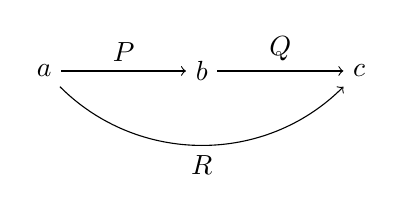
\begin{tikzpicture}
  \node (a) at (0,0) {$a$};
  \node (b) at (2,0) {$b$};
  \node (c) at (4,0) {$c$};
  
  \draw[->] (a) -- (b) node[midway, above] {$P$};
  \draw[->] (b) -- (c) node[midway, above] {$Q$};
  \draw[->, bend right=45] (a) to node[midway, below] {$R$} (c);
\end{tikzpicture}
\]
Note that if one assumes $\b>0$ then $\R = \P \diag(1/\b) \Q$.
%

The triangle inequality follows from
$$\begin{aligned}
\WassD_p(\a,\VectMode{c})&=\Big(\min_{\tilde\R\in \CouplingsD(\a,\VectMode{c})}\dotp{\tilde\R}{\distD^p}\Big)^{1/p} \leq \dotp{\R}{\distD^p}^{1/p}\\
&= \Big(\sum_{i,k}  \distD^p_{ik}\sum_{j} \S_{i,j,k} \Big)^{1/p} 
 \leq \Big(\sum_{i,j,k} \left(\distD_{ij}+\distD_{j,k}\Big)^p  \S_{i,j,k} \right)^{1/p} \\
& \leq \Big(\sum_{i,j,k} \distD^p_{ij} \S_{i,j,k} \Big)^{1/p} + \Big(\sum_{i,j,k}\distD^p_{j,k} \S_{i,j,k} \Big)^{1/p} \\
&= \Big(\sum_{i,j} \distD^p_{i,j}  \sum_k \S_{i,j,k} \Big)^{1/p} + \Big(\sum_{j,k} \distD^p_{j,k}  \sum_i \S_{i,j,k} \Big)^{1/p}\\
&= \Big(\sum_{i,j} \distD^p_{i,j}\P_{i,j}\Big)^{1/p} + \Big(\sum_{j,k} \distD^p_{j,k} \Q_{j,k}\Big)^{1/p} 
= \WassD_p(\a,\b) +\WassD_p(\b,\b).
\end{aligned}
$$
%
The first inequality is due to the sub-optimality of $\SS$, the second is the usual triangle inequality for elements in $\distD$, and the third comes from Minkowski's inequality.
\end{proof}

Proposition~\ref{prop-metric-histo} generalizes from histogram to arbitrary measures that need not be discrete. For this, one needs the following general gluing lemma.

\begin{lem}[Gluing lemma]\label{lem-gluing-general}
	Let $(\al,\be,\ga) \in \Mm_+^1(\Xx) \times \Mm_+^1(\Yy) \times \Mm_+^1(\Yy)$
	where $(\Xx,\Yy,\Zz)$ are three polish spaces (i.e. separable topological space which can be metrized using a distance which makes it a complete metric space).  
	%
	Given $\pi \in \Couplings(\al,\be)$ and $\xi \in \Couplings(\be,\ga)$, then there exists at least a tensor coupling measure
	$\sigma \in \Mm_+(\Xx \times \Yy \times \Zz)$ such that 
	\eq{
		(P_{\Xx,\Yy})_\sharp \sigma = \pi
		\qandq
		(P_{\Yy,\Zz})_\sharp \sigma = \xi
	}
	where we denoted the projector $P_{\Xx,\Yy}(x,y,z)=(x,y)$ and $P_{\Yy,\Zz}(x,y,z)=(y,z)$. 
\end{lem}
\begin{proof}
	The proof of this fundamental result is involved since it requires using the disintegration of measure (which corresponds to conditional probabilities). 
	%
	The disintegration of measures is applicable because the spaces are polish. 
	%
	We disintegrate $\pi$ and $\xi$ against $\be$ to obtain two families $(\pi_y)_{y \in \Yy}$ and $(\xi_y)_{y \in \Yy}$ of probability distributions on $\Xx$ and $\Zz$. These families are defined by the fact that 
	\eq{
		\foralls h \in \Cc(\Xx \times \Yy), \quad 
		\int_\Yy \Big( \int_\Xx h(x,y) \d \pi_y(x) \Big) \d \be(y) = \int h(x,y) \d\pi(x,y).
	}
	and similarly for $\xi$.
	%
	When $\be=\sum_i \b_j \de_{y_j}$ and $\pi=\sum_{i,j} \P_{i,j} \de_{y_j}$, then this conditional distribution is defined on the support of $\be$ as
	$\pi_{y_j} = \sum_i \frac{\P_{i,j}}{\b_j} \de_{x_i}$ (and similarly for $\xi$).
	%
	Then one defines the glued measure informally $``\sigma(x,y,z) = \pi_y(x) \xi_y(z) \be(y)''$, which formally reads
	\eq{
		\foralls g \in \Cc(\Xx \times \Yy \times \Zz), \quad
		\int g(x,y,z) \d\sigma(x,y,z) = \int g(x,y,z) \d \pi_y(x) \d \xi_y(z) \d \be(y).
	}
	For discrete measures, this matches the definition~\eqref{eq-glued-discr}, since $\sigma=\sum_{i,j,k} \S_{i,j,k} \de_{x_i,y_j,z_k}$ where
	\eq{
		\S_{i,j,k} = \frac{\P_{i,j}}{\b_j} \frac{\Q_{j,k}}{\b_j} \b_j.
	}
\end{proof}

Using this gluing lemma, we can now construct the Wasserstein distance in the general setting of arbitrary distributions on a Polish space.

\begin{prop}\label{prop-metric-measure}
We assume $\X=\Y$, and that for some $p \geq 1$, $\c(x,y)=\dist(x,y)^p$ where $\dist$ is a distance on $\X$, \emph{i.e.} \\
	\hbox{}\qquad (i) $\dist(x,y) = \dist(y,x) \geq 0$;  \\
	\hbox{}\qquad (ii)  $\dist(x,y)=0$ if and only if $x=y$;  \\
	\hbox{}\qquad (ii)  $\foralls (x,y,z) \in \X^3, \dist(x,z) \leq \dist(x,y)+\dist(y,z)$. \\
Then 
\eql{\label{eq-defn-wass-dist}
	\Wass_p(\al,\be) \eqdef \MK_{\dist^p}(\al,\be)^{1/p}
}
(note that $\Wass_p$ depends on $\dist$) defines the $p$-Wasserstein distance on $\X$, \emph{i.e.} $\Wass_p$ is symmetric, positive, $\Wass_p(\al,\be)=0$ if and only if $\al = \be$, and it satisfies the triangle inequality
\eq{
	\foralls (\al,\be,\ga) \in  \Mm_+^1(\X)^3, \quad \Wass_p(\al,\ga) \leq \Wass_p(\al,\be) + \Wass_p(\be,\ga).
}
\end{prop}

\begin{proof}
	The symmetry follows from the fact that since $d$ is symmetric, if $\pi(x,y)$ is optimal for $\MK_{\dist^p}(\al,\be)$, then 
	$\pi(y,x) \in \Couplings(\be,\al)$ is optimal for $\MK_{\dist^p}(\be,\al)$. 
	%
	If $\MK_{\dist^p}(\al,\be)=0$, then necessarily an optimal coupling $\pi$ is supported on the diagonal $\De \eqdef \{(x,x)\}_x \subset \Xx^2$.
	%
	We denote $\la(x)$ the corresponding measure on the diagonal, i.e. such that $\int h(x,y) \d\pi(x,y) = \int h(x,x) \d \la(x)$.
	%
	Then since $\pi \in \Couplings(\al,\be)$ necessarily $\la=\al$ and $\la=\be$ so that $\al=\be$.
	
	For the triangle inequality, we consider optimal couplings $\pi \in \Couplings(\al,\be)$ and $\xi \in \Couplings(\be,\ga)$
	and we glue them according to the Lemma~\ref{lem-gluing-general}.
	%
	We define the composition of the two couplings $(\pi,\xi)$ as $\rho \eqdef (P_{\Xx,\Zz})_\sharp \si$.
	%
	Note that if $\pi$ and $\xi$ are couplings induced by two Monge maps $T_\Xx(x)$ and $T_\Yy(y)$, then $\rho$ is itself induced by the Monge map $T_\Yy \circ T_\Xx$, so that this notion of composition of coupling generalizes the composition of maps.
	%
	The triangular inequality follows from  
	$$\begin{aligned}
		\Wass_p(\al,\ga) & \leq \Big( \int_{\Xx \times \Zz} \dist(x,z)^p \d\rho(x,z)\Big)^{1/p}  
		= \Big( \int_{\Xx \times \Yy \times \Zz} \dist(x,z)^p \d\si(x,y,z)\Big)^{1/p}		\\
		 &\leq \Big( \int_{\Xx \times \Yy \times \Zz} (\dist(x,y)+\dist(y,z))^p \d\si(x,y,z)\Big)^{1/p} \\
		 &\leq \Big( \int_{\Xx \times \Yy \times \Zz} \dist(x,y)^p \d\si(x,y,z)\Big)^{1/p}
		    +  \Big( \int_{\Xx \times \Yy \times \Zz} \dist(y,z)^p \d\si(x,y,z)\Big)^{1/p} \\
		  &= \Big( \int_{\Xx \times \Yy} \dist(x,y)^p \d\pi(x,y,z)\Big)^{1/p}
		    +  \Big( \int_{\Yy \times \Zz} \dist(y,z)^p \d\xi(y,z)\Big)^{1/p}
		    = \Wass_p(\al,\be)  + \Wass_p(\be,\ga) .
	\end{aligned}$$
\end{proof}

This distance $\Wass_p$ defined though Kantorovitch problem~\eqref{eq-defn-wass-dist} should be contrasted with the distance $\tilde\Wass$ obtained using Monge's problem~\eqref{eq-monge-distance}. Kantorovitch distance is always finite, while Monge's one might be infinite if the constraint set $\enscond{T}{T_\sharp \al=\be}$ is empty. One can show that as soon as this constraint set is non-empty, and even if no optimal $T$ exists, then one has $\Wass_p = \tilde\Wass_p$, which is a non-trivial result. Kantorovitch distance should thus be seen as a (convex) relaxation of Monge's distance, which behaves in a much nicer way, as we will explore next (it is continuous with respect to the convergence in law topology.


%%%%
\paragraph{Convergence in law topology.}

Let us first note that on a bounded metric space, all $\Wass_p$ distance defines the same topology (although they are not equivalent, the notion of converging sequence is the same).

\begin{prop}\label{prop-comp-wass-p}
	One has for $p \leq q$
	\eq{
		\Wass_p( \al,\be ) \leq \Wass_q(\al,\be) \leq \text{\upshape diam}(\Xx)^{\frac{q-p}{q}} \Wass_p(\al,\be)^{\frac{q}{p}}
	}
	where $\text{\upshape diam}(\Xx) \triangleq \usup{x,y} d(x,y)$.
\end{prop}
\begin{proof}
	The left inequality follows from Jensen inequality, $\phi(\int c(x,y) \d\pi(x,y)) \leq \int \phi(c(x,y)) \d\pi(x,y)$, applied to any probability distribution $\pi$ and to the convex function $\phi(r)=r^{q/p}$ to $c(x,y)=\norm{x-y}^p$, so that one gets
	\eq{
		\pa{\int \norm{x-y}^{p} \d\pi(x,y)}^{\frac{q}{p}} \leq \int \norm{x-y}^{q} \d\pi(x,y).
	} 	
	The right inequality follows from
	\eq{
		\norm{x-y}^q \leq \text{diam}(\Xx)^{q-p} \norm{x-y}^p.
	}
\end{proof}

The Wasserstein distance $\Wass_p$ has many important properties, the most important one being that it is a weak distance, \emph{i.e.} it allows to compare singular distributions (for instance discrete ones) and to quantify spatial shift between the supports of the distributions. This corresponds to the notion of weak$^*$ convergence.

\begin{defn}[Weak$^*$ topology]\label{dfn-weak-conv}
	$(\al_k)_k$ converges weakly$^*$ to $\al$ in $\Mm_+^1(\Xx)$ (denoted $\al_k \rightharpoonup \al$) if and only if for any continuous function $f \in \Cc(\Xx)$, $\int_\Xx f \d\al_k \rightarrow \int_\Xx f \d\al$.
\end{defn}

\begin{rem}[Weak$^*$ convergence for discrete measures]\label{rem-weak-conv-disc}
In the special case of a single Dirac, $\de_{x^{(n)}} \rightharpoonup \de_x$ is equivalent to $\int f \d\de_{x^{(n)}} = f(x^{(n)}) \rightarrow \int f \d\de_{x} = f(x)$ for any continuous $f$. This in turn is equivalent to $x^{(n)} \rightarrow x$. More generally, a sequence of discrete measures of the form $\al_n \eqdef \sum_k a_i^{(n)} \de_{ x_i^{(n)} }$ converges toward some measure $\sum_j b_j \de_{y_j}$ if and only if $a_i^{(n)} \rightarrow a_i$, and for those $a_i>0$, $x_i^{(n)} \rightarrow y_{\si(j)}$ for some injection $\si$ (in particular, the limit measure cannot have more point than the $\al_n$). Furthermore, one must also have the balance of mass $\sum_{i : \si(i)=j} a_i = b_j$ for all $j$.

\end{rem}

In terms of random vectors, if $X_n \sim \al_n$ and $X \sim \al$ (not necessarily defined on the same probability space), the weak$^*$ convergence corresponds to the convergence in law of $X_n$ toward $X$.

\begin{rem}[Central limit theorem]\label{rem-clt}
	The central limit theorem states that if $(X_1,\ldots,X_n)$ are i.i.d. distribution with finite second order moments, assuming $\EE(X_i)=0$ and $\EE(X_i X_i^\top)=\Id$, the rescaled average $Z_n \triangleq \frac{1}{\sqrt{n}} \sum_{i=1}^n X_i$ converges in law toward a Gaussian $\Nn(0,\Id)$. This means that the measure $\al_n$ representing the law of $Z_n$ converges weak$^*$ toward the measure $\al$ of the centered normalized Gaussian.
\end{rem}

\begin{defn}[Strong topology]
The simplest distance on Radon measures is the total variation norm, which is the dual norm of the $L^\infty$ norm on $\Cc(\Xx)$ and whose topology is often called the ``strong'' topology
\eq{
	\norm{\al-\be}_{\TV} \eqdef \usup{\norm{f}_\infty \leq 1} \int f \d(\al-\be)
	 = |\al-\be|(\Xx)
}
where $|\al-\be|(\Xx)$ is the mass of the absolute value of the difference measure. When $\al-\be=\rho \d x$ has a density, then $\norm{\al-\be}_{\TV}=\int |\rho(x)| \d x=\norm{\rho}_{L^1(\d x)}$ is the $L^1$ norm associated to $\d x$. When $\al-\be=\sum_i u_i \de_{z_i}$ is discrete, then $\norm{\al-\be}_{\TV}=\sum_i |u_i|=\norm{u}_{\ell^1}$ is the discrete $\ell^1$ norm. 
\end{defn}

The following proposition shows that the TV norm can be seen as a Wasserstein distance, but for a ``degenerate'' 0/1 metric.

\begin{prop}\label{prop-rel-wass-tv}
	Denoting $d$ the 0/1 distance such that $d(x,x)=0$ and $d(x,y)=1$ if $x \neq y$, then 
	\eq{
		\Wass_p(\al,\be)^p = \frac{1}{2}\norm{\al-\be}_{\TV}.
	}
\end{prop}
\begin{proof}
	For the sake of simplicity, we do the proof for discrete measures with weights $(\a,\b)$ and without loss of generality assume they have the same support $(x_i)_i$ and we denote $\D \triangleq (d(x_i,x_j))_{i,j}$ which is 0 on the diagonal and one outside. 
	%
	Also since $d^p=d$ we consider $p=1$. 
	We denote $\text{c}_i = \min(\a_i,\b_i)$.
	By conservation of mass, for $\P \in \CouplingsD(\a,\b)$, $\P_{i,i} \leq \text{c}_i$, thus
	\eq{
		\Wass_1(\al,\be) = \uinf{\P\ones=\a,\P^{\top}\ones=\b} \dotp{\P}{\D} = \sum_{i \neq j} \P_{i,j}
		= 1 - \sum_i \P_{i,i} = 1-\sum_i \text{c}_i.
	}
	We need to show that this bound is tight, namely to construct $\hat P \in \CouplingsD(\a,\b)$ such that 
	$\diag(\hat P)=\text{c}$. Let 
	\eq{
		\bar\a \triangleq \a-\text{c} = (\a-\b)_+ \geq 0
		\qandq
		\bar\b \triangleq \b-\text{c} = (\b-\a)_+ \geq 0
	}
	One has 
	\eq{
		\frac{ \bar a \otimes \bar b }{ \dotp{\bar a}{\ones} } \in \CouplingsD(\bar\a,\bar\b)
	}
	and we remark that $\dotp{\bar a}{\ones} = \dotp{\bar b}{\ones} = 1-\dotp{\text{c}}{\ones}$.
	%
	Thus denoting 
	\eq{
		\hat \P \triangleq \diag(\text{c}) + \frac{ \bar a \otimes \bar b }{ \dotp{\bar a}{\ones} } \in \CouplingsD(\bar\a,\bar\b) \geq 0
	}
	satisfies 
	\eq{
		\P \ones = \text{c} + \bar \a = \a
		\qandq
		\P^\top \ones = \text{c} + \bar \b = \b
	}
	so that $\hat P \in \CouplingsD(\a,\b)$  is a coupling so that $\diag(\hat P) = \diag(\text{c})$ since $\diag( \bar a \otimes \bar b )=0$. We thus conclude that
	\eq{
		\WassD_1(\a,\b) = \dotp{\D}{\hat \P} = 
		\sum_{i,j} \frac{\a_i\b_j}{\dotp{\bar a}{\ones}}
		= \sum_i \bar\a_i = \sum_i \bar\b_i = 
		= \frac{1}{2} \sum_i \bar\a_i + \bar\b_i
		= \frac{1}{2} \norm{\a-\b}_{\TV}.
	}
\end{proof}




As explained in Remark~\ref{rem-weak-conv-disc}, in the special case of Diracs, $\de_{x_n} \rightharpoonup \de_x$  is equivalent to $x_n \rightarrow x$. One can then contrast the strong topology with the Wasserstein distance if $x_n \neq x$, 
\eq{
	\norm{\de_{x_n}-\de_x}_{\TV}=2
	\qandq
	\Wass_p(\de_{x_n},\de_x) = d(x_n,x).
}
This shows that for the strong topology, Diracs never converge, while they do converge for the Wasserstein distance. It is a powerful property of the Wasserstein distance, which is regular with respect to the weak$^*$ topology, and metrizes it.

\begin{prop}
	If $\Xx$ is compact, $\al_k \rightharpoonup \al$ if and only if $\Wass_p(\al_k,\al) \rightarrow 0$. 
\end{prop}

The proof of this proposition requires the use of duality and is delayed to later, see Proposition~\ref{cor-topol-wass}. 
On non-compact spaces, one needs also to impose the convergence of the moments up to order $p$.
%
Note that there exist alternative distances which also metricize weak convergence. The simplest ones are Hilbertian kernel norms, which are detailed in Section~\ref{sec-dual-norms}.

Another example of such a weak convergence is the fact that on $\Xx=\RR$
\eq{
	\frac{1}{n} \sum_{k=1}^n \de_{k/n} \rightharpoonup \Uu_{[0,1]}
}
(convergence toward the uniform measure on $[0,1]$), which comes from the convergence of Riemann sums 
\eq{
	\foralls f \in \Cc(\RR), \quad
	\frac{1}{n} \sum_{k=1}^n f(k/n) \longrightarrow \int_0^1 f(x) \d x.
}
In the contrary, one has that for all $n$, since the two measures are mutually singular
\eq{
	\norm{ \frac{1}{n} \sum_{k=1}^n \de_{k/n} - \Uu_{[0,1]}}_{\TV} = 
	\norm{ \frac{1}{n} \sum_{k=1}^n \de_{k/n} }_{\TV} +  \norm{\Uu_{[0,1]}}_{\TV} = 2
}
so that there is no strong convergence.

On discrete space, the strong and the weak topology coincide, and the following proposition relates the TV and Wasserstein distance together. 

\begin{prop}
	One has
	\eq{
		\frac{d_{\min}}{2}\norm{\al-\be}_{\TV} \leq \Wass_1(\al,\be) \leq \frac{d_{\max}}{2}  \norm{\al-\be}_{\TV} 
		\qwhereq
		\choice{
			d_{\min} \eqdef \uinf{x \neq y} d(x,y) \\
			d_{\max} \eqdef \usup{x,y} d(x,y)
		}
	}
\end{prop}

\begin{proof}
	We denote $d_0(x,y)$ the distance such that $d_0(x,x)=0$ and $d_0(x,y)=1$ for $x \neq y$. One has 
	\eq{
		d_{\min} d_0(x,y) \leq d(x,y) \leq d_{\max} d_0(x,y)
	}
	so that integrating this against any $\pi \in \Couplings(\al,\be)$ and taking the minimum among those $\pi$ gives the result using Proposition~\eqref{prop-rel-wass-tv}. 
\end{proof}

This bound is sharp, as this can be observed by taking $\al=\de_{x}$ and $\be=\de_y$, in which case the bound simply reads if $x \neq y$
\eq{
	d_{\min} \leq d(x,y) \leq d_{\max}. 
}
%
This shows that the ratio between the two distances can blow as $d_{\max}/d_{\min}$ increases, and on non-discrete space, if $d_{\min}=0$, then the two distances are not equivalent, which is inlined with the fact that the strong and the weak topology do not coincide. 



\begin{rem}[Berry-Esseen theorem]
The Wasserstein distance is a natural candidate to quantify the convergence in law in the central limit theorem (Remark~\ref{rem-clt}). To obtain rates, one needs further assumption on the random vector, and the Berry-Esseen theorem ensures that if $\EE(\norm{X_i}^3)<+\infty$, then $\Wass_p(\al_k,\al) = O(\EE(\norm{X_i}^3)/\sqrt{n})$.
\end{rem}
 
 
%%%%%
\paragraph{Applications and implications}

Applications for having a geometric distance: barycenters, shape registration loss functions, density fitting.
%
The typical setup is to fit a parametric measure $\th \mapsto \al_\th$ to an (empirical) measure $\be$ by minimizing the function $\th \mapsto \Wass_p(\al_\th,\be)$.




% !TEX root = ../CourseOT.tex


%%%%%%%%%%%%%%%%%%%%%%%%%%%%%%%%%%%%%%%%%%%%%%%%%%%%%%%%%%%%%%%%%%%%%%%%%%%
%%%%%%%%%%%%%%%%%%%%%%%%%%%%%%%%%%%%%%%%%%%%%%%%%%%%%%%%%%%%%%%%%%%%%%%%%%%
%%%%%%%%%%%%%%%%%%%%%%%%%%%%%%%%%%%%%%%%%%%%%%%%%%%%%%%%%%%%%%%%%%%%%%%%%%%
\section{Sinkhorn}

%%%%%%%%%%%%%%%%%%%%%%%%%%%%%%%%%%%%%%%%%%%%%%%%%%%%%%%%%%%%%%%%%%%%%%%%%%%
\subsection{Entropic Regularization for Discrete Measures}


%%%%%
\paragraph{Entropic Regularization for Discrete Measures.}

The idea of the entropic regularization of optimal transport is to use the Shannon-Boltzmann entropy
\eq{
	\HD(\P) \triangleq -\sum_{i,j} \P_{i,j} \log(\P_{i,j}), 
} 
with the convention $0 \log(0)$
as a regularizing function to obtain approximate solutions to the original transport problem~\eqref{eq-kanto-discr} 
\eql{\label{eq-regularized-discr}
	\MKD_\C^\epsilon(\a,\b) \eqdef 
	\umin{\P \in \CouplingsD(\a,\b)}
		\dotp{\P}{\C} - \epsilon \HD(\P).
} 
This is a strictly convex optimization problem. 
%
Indeed, the function $-\HD$ is strongly convex, because its hessian is $-\partial^2 \HD(\P)=\diag(1/\P_{i,j})$ and $\P_{i,j} \leq 1$. 



%%%%%
\paragraph{Smoothing effect.}

Since the objective is a $\epsilon$-strongly convex function, problem~\ref{eq-regularized-discr} has a unique optimal solution. 
%
This smoothing, beyond providing uniqueness, actually leads to $\MKD_\C^\epsilon(\a,\b)$ being a smooth function of $\a, \b$ and $\C$. \todo{detail this, make a section}
%
The effect of the entropy is to act as a barrier function for the positivity constraint. As we will show later, this forces the solution $\P$ to be strictly positive on the support of $\a \otimes \b$. We will also show that as $\epsilon\to+\infty$, then the solution $\P \to \a \otimes \b$




%%%%%%%%%%%%%%%%%%%%%%%%%%%%%%%%%%%%%%%%%%%%%%%%%%%%%%%%%%%%%%%%%%%%%%%%%%%
\subsection{Sinkhorn's Algorithm}

The following proposition shows that the solution of~\eqref{eq-regularized-discr} has a specific form, which can be parameterized using $n+m$ variables. That parameterization is therefore essentially dual, in the sense that a coupling $\P$ in $\CouplingsD(\a,\b)$ has $nm$ variables but $n+m$ constraints.

\begin{prop}\label{prop-regularized-primal}
$\P$ is the unique solution to~\eqref{eq-regularized-discr} if and only if there exists  $(\uD,\vD) \in \RR_+^n \times \RR_+^m$ such that 
\eql{\label{eq-scaling-form}
	\foralls (i,j) \in \range{n} \times \range{m}, \quad \P_{i,j} = \uD_i \K_{i,j} \vD_j
	\qwhereq \K_{i,j} \eqdef e^{-\frac{-\C_{i,j}}{\epsilon}}, 
}
and $\P \in \Couplings(\a,\b)$.
\end{prop} 

\begin{proof}
Without loss of generality, we assume $\a_i,\b_j>0$ (otherwise, we can set the corresponding $\uD_i$ or $\vD_j$ to 0).

The first thing to prove is that if $\P^\star$ is the solution (which is unique by strict convexity of the entropy) then $\P_{i,j}^\star>0$ for all $(i,j)$. Indeed, if $\P_{i,j}^\star=0$, then we can consider $\P_t = (1-t)\P^\star + t \a \otimes \b$, which satisfies the marginal constraint and is positive for $t \in [0,1]$ small enough. One then check that, denoting $\Ee(\P) \eqdef \dotp{\P}{\C}+\H(\P)$ the objective function, and $f(t) \eqdef \Ee(\P_t)$, then $f'(0) = -\infty$, so that for $t$ small enough, $\Ee(\P_t)<\Ee(\P^\star)$ which is a contradiction.

We can thus ignore the positivity constraint when introducing two dual variables $\fD\in\RR^n,\gD\in\RR^m$ for each marginal constraint so that the Lagrangian of~\eqref{eq-regularized-discr} reads
\eq{\label{eq-sinkhorn-lagrangian}
	\Lag(\P,\fD,\gD)= \dotp{\P}{\C} + \epsilon H(\P) + \dotp{\fD}{\a - \P\ones_m} + \dotp{\gD}{\b - \transp{\P}\ones_n}.
}
Considering first-order conditions (where we ignore the positivity constraint as explained above), we have
$$
	\frac{\partial\Lag(\P,\fD,\gD)}{\partial \P_{i,j}}= \C_{i,j} + \epsilon (\log\pa{ \P_{i,j} }+1) - \fD_i -\gD_j = 0.
$$
which results, in an optimal $\P$ coupling of the regularized problem, in the expression 
$\P_{i,j}=e^{\frac{\fD_i+\gD_j - \C_{i,j}}{\epsilon}-1}$ 
which can be rewritten in the form provided in the proposition using non-negative vectors $\uD \eqdef (e^{\fD_i/\varepsilon}-1)_i$ and $\vD \eqdef (e^{\gD_j/\varepsilon})_j$.
\end{proof} 

The factorization of the optimal solution exhibited in Equation~\eqref{eq-scaling-form} can be conveniently rewritten in matrix form as $\P=\diag(\uD)\K\diag(\vD)$.
%
$\uD,\vD$ must therefore satisfy the following non-linear equations which correspond to the mass conservation constraints inherent to $\CouplingsD(\a,\b)$,
\eql{\label{eq-dualsinkhorn-constraints}
	\diag(\uD)\K\diag(\vD)\ones_m=\a,
	\qandq
	\diag(\vD)\K^\top \diag(\uD)\ones_n=\b,
}
These two equations can be further simplified, since $\diag(\vD)\ones_m$ is  $\vD$, and the multiplication of $\diag(\uD)$ times $\K \vD$ is 
\eql{\label{eq-dualsinkhorn-constraints2}
	\uD \odot (\K \vD) = \a
	\qandq
	\vD \odot (\transp{\K}\uD) = \b
}
where $\odot$ corresponds to the entry-wise multiplication of vectors. This problem is known in the numerical analysis community as the matrix scaling problem (see~\cite{nemirovski1999complexity} and references therein).

The problem of normalizing a positive matrix $\K$ by diagonal scaling is well known, in particular when $n=m$ and $\a$ and $\b$ are uniform. This corresponds to the question of diagonal scaling toward bi-stochasticity, which is a very old problem. The previous result shows that there is a unique such scaled matrix $\P$, thanks to the strong convexity of the regularized problem. However, the question remains to find in practice this scaled matrix. Note also that if some entry of $\K$ vanish (or equivalently if the cost matrix $\C$ can have infinite values)


An intuitive way to try to solve these equations is to solve them iteratively, by modifying first $\uD$ so that it satisfies the left-hand side of Equation~\eqref{eq-dualsinkhorn-constraints2} and then $\vD$ to satisfy its right-hand side. These two updates define Sinkhorn's algorithm
\eql{\label{eq-sinkhorn}	
	\itt{\uD} \eqdef \frac{\a}{\K \it{\vD}}
	\qandq
	\itt{\vD} \eqdef \frac{\b}{\transp{\K}\itt{\uD}},
}
initialized with an arbitrary positive vector, for instance $\init{\vD} = \ones_m$. The division operator used above between two vectors is to be understood entry-wise. Note that a different initialization will likely lead to a different solution for $\uD,\vD$, since $\uD,\vD$ are only defined up to a multiplicative constant (if $\uD,\vD$ satisfy \eqref{eq-dualsinkhorn-constraints} then so do $\lambda\uD,\vD/\lambda$ for any $\lambda>0$).
%
It turns out however that these iterations converge, as we detail next. 

A chief advantage, besides its simplicity, of Sinkhorn's algorithm is that the only computationally expensive step is matrix-vector multiplication by the Gibbs kernel so that its complexity scales like $C nm$ where $C$ is the number of Sinkhorn iteration, which can be shown to be of the order $1/\epsilon^2$ f one is interested in reaching an accuracy $\epsilon$ on the (unregularized) transportation cost. Note however that in many situations, one is not interested in reaching high accuracy, because targeted application success is often only remotely connected to the ability to solve an optimal transport problem (but rather only being able to compare in a geometrically faithful way distribution), so that $K$ is usually quite small.
%
This should be contrasted with interior point methods, which also operate by introducing a barrier function of the form $-\sum_i \log(\P_{i,j})$. These algorithms have typically a complexity of the order $O(n^6 \log(|\epsilon|))$. 

The second crucial aspect of Sinkhorn is that matrix-vector multiplication streams extremely well on GPU. Even better, if one is interested in computing many OT problems with a fixed cost matrix $\C$, one can replace many matrix-vector multiplications with matrix-matrix multiplications, so that the computation gain is enormous. 



%%%%%%%%%%%%%%%%%%%%%%%%%%%%%%%%%%%%%%%%%%%%%%%%%%%%%%%%%%%%%%%%%%%%%%%%%%%
\subsection{Reformulation using relative entropy}

A convenient tool to re-formulate and ``normalize'' this discrete entropy (which is crucial to formulate a continuous version of the problem below) is to consider the relative entropy, also called  Kullback-Leibler divergence, which is defined as
\eql{\label{eq-kl-defn}
	\KLD(\P|\Q) \eqdef \sum_{i,j}  \P_{i,j} \log\pa{\frac{\P_{i,j}}{\Q_{i,j}}} - \P_{i,j} + \Q_{i,j}.
}
with the convention $0\log(0)=0$ and $\KLD(\P|\Q)=+\infty$ if there exists some $(i,j)$ such that $\Q_{i,j}=0$ but $\P_{i,j} \neq 0$. 
%
For the specific case of comparing probability distribution, this further simplifies to 
\eq{
	\KLD(\P|\Q) = \sum_{i,j}  \P_{i,j} \log\pa{\frac{\P_{i,j}}{\Q_{i,j}}}.
}
The Shannon-Boltzmann neg-entropy is obtained when considering $\Q=\ones_{n \times m}$, i.e.  
\eq{
	\HD( \P ) = -\KLD(\P|\ones_{n \times m}).
}
$\KLD$ is a particular instance (and the unique case) of both a $\phi$-divergence (as defined in Section~\ref{sec-phi-div}) and a Bregman divergence. This unique property is at the heart of the fact that this regularization leads to elegant algorithms and a tractable mathematical analysis. One thus has $\KLD(\P|\Q) \geq 0$ and  $\KLD(\P|\Q)=0$ if and only if $\P=\Q$ (see Proposition~\ref{phi-div-positive}).
%
Indeed, it reads
\eq{
	\KLD(\P|\Q) = \sum_{i,j}  \phi( \P_{i,j} / \Q_{i,j} ) \Q_{i,j}.
}
where $\phi(s)=s\log(s)$. For any convex $\phi$ such that $\phi(1)=0$, one has indeed by Jensen
\eq{
	\sum_{i,j}  \phi( \P_{i,j} / \Q_{i,j} ) \Q_{i,j} \geq \phi( \sum_{i,j}  \P_{i,j} / \Q_{i,j}  \Q_{i,j}  )
	= \phi( \sum_{i,j} \P_{i,j} ) =\phi(1)= 0. 
}

For instance, one can use as reference measure the tensor product $\a \otimes \b = (\a_i \b_j)_{i,j}$ and consider 
\eql{\label{eq-regularized-discr-rescaled}
	\umin{\P \in \CouplingsD(\a,\b)}
		\dotp{\P}{\C} - \epsilon \KL(\P|\a \otimes \b).
} 
Note also that for later, it will be important to have this normalization when considering unbalanced OT (see Section~\ref{sec-unbalanced}).

But, the choice of normalization (i.e. reference measure), has no importance for the selection of the optimal $\P$ since it only affects the objective by a constant, as shown in the following proposition.
%
In particular,~\eqref{eq-regularized-discr-rescaled} and~\eqref{eq-regularized-discr} have the same unique solution.


\begin{prop} \label{prop-kl-shift} For $\P \in \CouplingsD(\a,\b)$, one has
\eq{
	\KLD(\P|\a \otimes \b) = 
	\KLD(\P|\a' \otimes \b') - \KLD(\a|\a') - \KL(\b|\b').
} 
\end{prop}

\begin{proof}
This follows from 
\eq{
	\sum_{i,j} \P_{i,j} \log\frac{\P_{i,j}}{\a_i\b_j}
	= 
	\sum_{i,j} \P_{i,j} \log\frac{\P_{i,j}}{\a_i'\b_j'}
	+ 
	\sum_{i,j} \P_{i,j} \pa{\log\frac{\a_i'}{\a_i} + \log\frac{\b_j'}{\b_j}}.
} 
\end{proof}

The choice of using the reference measure $\a \otimes \b$ is however important to deal with situations where the support of $\a$ and $\b$ can change (so that some coordinate of $\a$ or $\b$ might vanish), and more importantly in the following section which deals with possibly continuous distributions. 


One has the following convergence property.
 
\begin{prop}[Convergence with $\epsilon$]\label{prop-convergence-eps}
The unique solution $\P_\epsilon$ of~\eqref{eq-regularized-discr} converges to the optimal solution with maximal entropy within the set of all optimal solutions of the Kantorovich problem, namely
\eql{\label{eq-entropy-conv-1}
	\P_\epsilon \overset{\epsilon \rightarrow 0}{\longrightarrow}
	\uargmin{\P} \enscond{ -\HD(\P) }{
		\P \in \CouplingsD(\a,\b), \dotp{\P}{\C} = \MKD_\C(\a,\b)
	}
}
so that in particular
\eq{
	\MKD_\C^\epsilon(\a,\b) \overset{\epsilon \rightarrow 0}{\longrightarrow} \MKD_\C(\a,\b).
}
One has
\eql{\label{eq-entropy-conv-2}
	\P_\epsilon \overset{\epsilon \rightarrow \infty}{\longrightarrow}
	\a \otimes \b.
}
\end{prop}

\begin{proof}
	\textbf{Case $\epsilon \rightarrow 0$.}
	 We consider a sequence $(\epsilon_\ell)_\ell$ such that $\epsilon_\ell \rightarrow 0$ and $\epsilon_\ell > 0$.	
 	We denote $\P_\ell$ the solution of~\eqref{eq-regularized-discr} for $\epsilon=\epsilon_\ell$. 
	%
	Since $\CouplingsD(\a,\b)$ is bounded, we can extract a sequence (that we do not relabel for the sake of simplicity) such that $\P_\ell \rightarrow \P^\star$. Since $\CouplingsD(\a,\b)$ is closed, $\P^\star \in \CouplingsD(\a,\b)$. We consider any $\P$ such that $\dotp{\C}{\P} = \MKD_\C(\a,\b)$. By optimality of $\P$ and $\P_\ell$ for their respective optimization problems (for $\epsilon=0$ and $\epsilon=\epsilon_\ell$), one has
 	\eql{\label{eq-proof-gamma-conv}
 		0 \leq \dotp{\C}{\P_\ell} - \dotp{\C}{\P} \leq \epsilon_\ell ( \KLD(\P_\ell|\a \otimes \b)-\KLD(\P|\a \otimes \b) ).
 	}
 	Since $\KLD$ is continuous, taking the limit $\ell \rightarrow +\infty$ in this expression shows that 
 	$\dotp{\C}{\P^\star} = \dotp{\C}{\P}$ so that $\P^\star$ is a feasible point of~\eqref{eq-entropy-conv-1}. Furthermore, dividing by $\epsilon_\ell$ in~\eqref{eq-proof-gamma-conv} and taking the limit shows that 
 	$\KLD(\P|\a \otimes \b) \leq \KLD(\P^\star|\a \otimes \b)$, which shows that $\P^\star$ is a solution of~\eqref{eq-entropy-conv-1}. Since the solution $\P_0^\star$ to this program is unique by strict convexity of $\KLD(\cdot|\a \otimes \b)$, one has $\P^\star = \P_0^\star$, and the whole sequence is converging. 
	
	
	\textbf{Case $\epsilon \rightarrow +\infty$.} Evaluating at $\a \otimes \b$ (which belongs to the constraint set $\CouplingsD(\a,\b)$) the energy, one has
	\eq{
		\dotp{\C}{\P_\epsilon} + \epsilon \KLD(\P_\epsilon|\a \otimes \b) \leq \dotp{\C}{\a \otimes \b} + \epsilon \times 0
	}
	and since $\dotp{\C}{\P_\epsilon} \geq 0$, this leads to
	\eq{
		\KLD(\P_\epsilon|\a \otimes \b) \leq \epsilon^{-1} \dotp{\C}{\a \otimes \b} \leq \frac{\norm{\C}_\infty}{\epsilon}
	}
	so that $\KLD(\P_\epsilon|\a \otimes \b) \rightarrow 0$ and thus $\P_\epsilon \rightarrow \a \otimes \b$ since $\KLD$ is a valid divergence.
\end{proof}




%%%%%%%%%%%%%%%%%%%%%%%%%%%%%%%%%%%%%%%%%%%%%%%%%%%%%%%%%%%%%%%%%%%%%%%%%%%
\subsection{General Formulation}

One can consider arbitrary measures by replacing the discrete entropy with the relative entropy with respect to the product measure $\d\al\otimes\d\be(x,y) \eqdef \d\al(x)\d\be(y)$, and propose a regularized counterpart to~\eqref{eq-mk-generic} using
\eql{\label{eq-entropic-generic}
	\MK_\c^\epsilon(\al,\be) \eqdef 
	\umin{\pi \in \Couplings(\al,\be)}
		\int_{X \times Y} c(x,y) \d\pi(x,y) + \epsilon \KL(\pi|\al\otimes\be)
}
where the relative entropy is a generalization of the discrete Kullback-Leibler divergence~\eqref{eq-kl-defn}
\eql{\label{eq-defn-rel-entropy}
	\KL(\pi|\xi) \eqdef \int_{\X \times \Y} \log\Big( \frac{\d \pi}{\d\xi}(x,y) \Big) \d\pi(x,y)
	  + \int_{\X \times \Y} (\d\xi(x,y)-\d\pi(x,y)), 
}
and by convention $\KL(\pi|\xi)=+\infty$ if $\pi$ does not have a density $\frac{\d \pi}{\d\xi}$ with respect to $\xi$. 
%
It is important to realize that the reference measure $\al\otimes\be$ chosen in~\eqref{eq-entropic-generic} to define the entropic regularizing term $\KL(\cdot|\al\otimes\be)$ plays no specific role (because Proposition~\ref{prop-kl-shift} still applies in this general setting), only its support matters.
%
This problem is often referred to as the ``static Schr\"odinger problem'', since $\pi$ is intended to model the most likely coupling between particles of gas which can be only observed at two different times (it is the so-called lazy gaz model). The parameter $\epsilon$ controls the temperature of the gas, and particles do not move in a deterministic straight line as in optimal transport for the Euclidean cost, but rather according to a stochastic Brownian bridge. 

\begin{rem}[Probabilistic interpretation]
	If $(X,Y) \sim \pi$ have marginals $X \sim \al$ and $Y \sim \be$, then $\KL(\pi|\al \otimes \be) = \Ii(X,Y)$ is the mutual information of the couple, which is 0 if and only if $X$ and $Y$ are independent. The entropic problem~\eqref{eq-entropic-generic} is thus equivalent to
	\eq{
		\umin{(X,Y), X \sim \al, Y \sim \be } \EE( c(X,Y)) + \epsilon \Ii(X,Y). 
	}
	Using a large $\epsilon$ thus enforces the optimal coupling to describe independent variables, while, according to Brenier's theorem, small $\epsilon$ rather imposes a deterministic dependency between the couple according to a Monge map. 
\end{rem}


%%%%%%%%%%%%%%%%%%%%%%%%%%%%%%%%%%%%%%%%%%%%%%%%%%%%%%%%%%%%%%%%%%%%%%%%%%%
\subsection{Convergence of Sinkhorn}
\label{sec-convergence-init}

This section provides a first overview of convergence proof for Sinkhorn. For the sake of simplicity, this section is written for discrete measures, but the analysis carries over to general measures. This analysis is revisited in Section~\ref{sec-convergence-dual} using convex duality. 

%%%%
\paragraph{Alternating $\KL$ projections.}

The following proposition explains that the minimized objective is equal to a KL distance toward the Gibbs distribution.

\begin{prop} 
One has 
\eq{
	\dotp{\P}{\C} + \epsilon \KLD(\P|\a \otimes \b) = \epsilon \KLD(\P|\K) + \text{cst}, 
}
\end{prop}
\begin{proof}
The objective is indeed equal to
\eq{
	\epsilon \sum_{i,j} \P_{i,j} \frac{\C_{i,j}}{\epsilon} + \log\pa{\frac{\P_{i,j}}{\a_i \b_j}} \P_{i,j}
	 = \epsilon \sum_{i,j} \P_{i,j} \log\pa{\frac{\P_{i,j}}{\a_i \b_j e^{-\C_{i,j}/\epsilon}}} 
	 = \epsilon \sum_{i,j} \P_{i,j} \log\pa{\frac{\P_{i,j}}{\K_{i,j}}}
	 + \text{cst}.
}
\end{proof}

This shows that the unique solution $\P_\epsilon$ of~\eqref{eq-regularized-discr} is a projection onto $\CouplingsD(\a,\b)$ of the Gibbs kernel $\K$
\eql{\label{eq-kl-proj}
	\P_\epsilon = \Proj_{\CouplingsD(\a,\b)}^\KLD(\K) \eqdef \uargmin{\P \in \CouplingsD(\a,\b)} \KLD(\P|\K).
}

Denoting 
\eq{
	\Cc^1_\a \eqdef \enscond{\P}{\P\ones_m=\a}
	\qandq
	\Cc^2_\b \eqdef \enscond{\P}{\transp{\P}\ones_m=\b}
}
the rows and columns constraints, one has $\CouplingsD(\a,\b) = \Cc^1_\a \cap \Cc^2_\b$. One can use Bregman iterative projections~\cite{bregman1967relaxation}
\eql{\label{eq-kl-sinkh-proj}
	\itt{\P} \eqdef \Proj_{\Cc^1_\a}^{\KLD}(\it{\P})
	\qandq
	\ittt{\P} \eqdef \Proj_{\Cc^2_\b}^{\KLD}(\itt{\P}).
}
Since the sets $\Cc^1_\a$ and $\Cc^2_\b$ are affine, these iterations are known to converge to the solution of~\eqref{eq-kl-proj}, see~\cite{bregman1967relaxation}. 

The two projectors are simple to compute since they correspond to scaling respectively the rows and the columns, as explained in this proposition.

\begin{prop}
One has 
\eq{
	 \Proj_{\Cc^1_\a}^{\KLD}(\P) = \diag\pa{\frac{\a}{\P \ones_m}} \P
	 \qandq
	 \Proj_{\Cc^2_\b}^{\KLD}(\P) =  \P \diag\pa{\frac{\b}{\P^\top \ones_n}}.
}
\end{prop}
\begin{proof}
	One considers the problem along each row or column vector to impose a fixed sum $s \in \RR_+$
	\eq{
		\umin{p} \enscond{ \KL(p|q) }{ \dotp{p}{\ones}=s }.
	}
	The Lagrange multiplier for this problem read
	\eq{
		\log(p/q)+\la \ones=0 \qarrq
		p = u q \qwhereq u = e^{-\la}>0.
	}
	One has $\dotp{p}{\ones} = s$ which is equivalent to $\dotp{uq}{\ones}=s$ i.e. $u=s/\sum_i q_i$ and hence the desired scaling resulting formula 
	$p=s p/\sum_i q_i$. 
\end{proof}

These iterations are equivalent to Sinkhorn iterations~\eqref{eq-sinkhorn} since defining 
\eq{\label{eq-sink-matrix}\P^{(2\ell)} \eqdef \diag(\it{\uD}) \K \diag(\it{\vD}),}
one has
\begin{align*}
	\P^{(2\ell+1)} &\eqdef \diag(\itt{\uD}) \K \diag(\it{\vD}) \\
	\qandq
	\P^{(2\ell+2)} &\eqdef \diag(\itt{\uD}) \K \diag(\itt{\vD})
\end{align*}
In practice however one should prefer using~\eqref{eq-sinkhorn} which only requires manipulating scaling vectors and multiplication against a Gibbs kernel, which can often be accelerated. \todo{ (see below Remarks~\ref{rem-separable} and~\ref{rem-geod-heat}). }

Such a convergence analysis using Bregman projection is however of limited interest because it only works in finite dimension. For instance, the linear convergence speed one can obtain with these analyses (because the objective is strongly convex) will degrade with the dimension (and also with $\epsilon$). 
%
It is also possible to decay $\epsilon$ during the iterates to improve the speed and rely on multiscale strategies in low dimensions.
 
% \todo{Remark on Bregman divergence, generalization of projected gradient desc (mirror descent), etc.}



%%%%
\paragraph{Convergence for the Hilbert metric}

As initially explained by~\cite{franklin1989scaling}, the global convergence analysis of Sinkhorn is greatly simplified using Hilbert projective metric on $\RR_{+,*}^n$ (positive vectors), defined as
\eq{
	\foralls (\uD,\uD') \in (\RR_{+,*}^n)^2, \quad
	\Hilbert(\uD,\uD') \eqdef 
	\norm{\log(\uD)-\log(\vD)}_V
}
where the variation semi-norm is
\eq{
	\norm{z}_V = \max(z)-\min(z).
}
One can show that $d_\Hh$ is a distance on the projective cone $\RR_{+,*}^n/\sim$, where $\uD \sim \uD'$ means that $\exists s>0, \uD=s\uD'$ (the vector are equal up to rescaling, hence the naming ``projective''), and that $(\RR_{+,*}^n/\sim,d_\Hh)$ is then a complete metric space.  
%
It was introduced independently by~\cite{birkhoff1957extensions} and~\cite{samelson1957perron} to provide quantitative proof of the Perron-Frobenius theorem (convergence of iterations of positive matrices). Sinkhorn should be thought as a non-linear generalization of Perron-Frobenius. 


\begin{thm}\label{thm-birkoff}
	Let $\K \in \RR_{+,*}^{n \times m}$, then for $(\vD,\vD') \in (\RR_{+,*}^m)^2$
	\eq{
		\Hilbert(\K \vD,\K \vD') \leq \la(\K) \Hilbert(\vD,\vD')
		\text{ where }
		\choice{
			\la(\K) \eqdef \frac{ \sqrt{\eta(\K)}-1 }{ \sqrt{\eta(\K)}+1 } < 1 \\
			\eta(\K) \eqdef \umax{i,j,k,\ell} \frac{ \K_{i,k} \K_{j,\ell} }{ \K_{j,k} \K_{i,\ell} }.
		}
	}
\end{thm}

Note that this results extends to arbitrary convex cones and affine mapping from the cone to its interior, with the 

The following theorem proved by~\cite{franklin1989scaling}, makes use of this Theorem~\ref{thm-birkoff} to show the linear convergence of Sinkhorn's iterations.

\begin{thm}
	One has $(\it{\uD},\it{\vD}) \rightarrow (\uD^\star,\vD^\star)$ and
	\eql{\label{eq-convlin-sinkh}
		\Hilbert(\it{\uD}, \uD^\star) = O(\la(\K)^{2\ell}), \quad
		\Hilbert(\it{\vD}, \vD^\star) = O(\la(\K)^{2\ell}).
	}
	One also has
	\eql{\label{eq-convsinkh-control}
		\Hilbert(\it{\uD}, \uD^\star) \leq \frac{\Hilbert( \it{\P}\ones_m,\a )}{1-\la(\K)} 
		\qandq
		\Hilbert(\it{\vD}, \vD^\star) \leq \frac{\Hilbert( \P^{(\ell),\top} \ones_n,\b )}{1-\la(\K)}, 
	}
	where we denoted $\it{\P} \eqdef \diag(\it{\uD}) \K \diag(\it{\vD})$. Lastly, one has
	\eql{\label{eq-convlin-sinkh-prim}
		\|\log(\it{\P}) - \log(\P^\star)\|_\infty \leq \Hilbert(\it{\uD}, \uD^\star) + \Hilbert(\it{\vD}, \vD^\star)
	}
	where $\P^\star$ is the unique solution of~\eqref{eq-regularized-discr}. 
\end{thm}

\begin{proof}
	One notice that for any $(\vD,\vD') \in (\RR_{+,*}^m)^2$, one has 
	\eq{	
		\Hilbert(\vD,\vD') = \Hilbert(\vD/\vD',\ones_m) = \Hilbert(\ones_m/\vD,\ones_m/\vD'), 
	}
	since indeed $\Hilbert(\a/\vD,\a/\vD') = \Hilbert(\vD,\vD')$.
	%
	This shows that
	\begin{align*}
		\Hilbert(\itt{\uD},\uD^\star) &= \Hilbert\pa{ \frac{\a}{\K \it{\vD}}, \frac{\a}{\K \vD^\star} } 
		= \Hilbert( \K \it{\vD}, \K \vD^\star ) \leq \la(\K) \Hilbert( \it{\vD}, \vD^\star ).
	\end{align*}
	where we used Theorem~\ref{thm-birkoff}. This shows~\eqref{eq-convlin-sinkh}.  One also has, using the triangular inequality
	\begin{align*}
		\Hilbert(\it{\uD},\uD^\star) &\leq \Hilbert(\itt{\uD},\it{\uD}) + \Hilbert(\itt{\uD},\uD^\star) 
		\leq \Hilbert\pa{ \frac{\a}{\K \it{\vD}},\it{\uD} } + \la(\K) \Hilbert(\it{\uD},\uD^\star) \\
		&= \Hilbert\pa{ \a,\it{\uD} \odot  ( \K \it{\vD} ) } + \la(\K) \Hilbert(\it{\uD},\uD^\star), 
	\end{align*}
	which gives the first part of~\eqref{eq-convsinkh-control} since 
	$\it{\uD} \odot  ( \K \it{\vD} ) = \it{\P}\ones_m$ (the second one being similar).
	%
	The proof of~\eqref{eq-convlin-sinkh-prim} follows from~\cite[Lemma 3]{franklin1989scaling}
\end{proof}
 
The bound~\eqref{eq-convsinkh-control} shows that some error measures on the marginal constraints violation, for instance, $\| \it{\P} \ones_m - \a \|_1$ and $\|\transp{\it{\P}} \ones_n - \b \|_1$, are useful stopping criteria to monitor the convergence. 
%
This theorem shows that the Sinkhorn algorithm converges linearly, but the rates become exponentially bad as $\epsilon \rightarrow 0$, since it scales like $e^{-\norm{c}_\infty/\epsilon}$. In practice, one eventually observes a linear rate after enough iteration, because the local linear rate is much better, usually of the order $1-\epsilon$. 
%
Note also that while we wrote the proof for discrete measures, they carry over without modification to arbitrary measures. 
%
But an important limitation of this analysis is that it is restricted to compactly supported measures, since the cost needs to be uniformly bounded (for instance, analyzing Gaussian distribution requires a different approach).   

\input{sections/dual}
\input{sections/semidiscr-w1}
\input{sections/dual-norms}
\input{sections/sinkhorn-div}
%\input{sections/barycenters}
%\input{sections/estimation}
%% !TEX root = ../CourseOT.tex

\section{Wasserstein (gradient) Flows}

The goal of this section is to expose the connection between optimal transport and certain evolutions over the space of probability distributions, particularly solutions to some PDEs and generative models using diffusion. The exposition is informal, focusing on intuition rather than rigorous proof. We work over the space $\mathcal{X} = \mathbb{R}^d$. It is also the opportunity to draw connexion with recent applications in ML, most notably analyzing the training dynamic of MLP, modeling deep transformers, and flow matching for generative models.

\subsection{Evolutions over the Space of Measures}

We consider the evolution $t \mapsto \alpha_t \in \mathcal{P}(\mathbb{R}^d)$. Such evolution can be described in a ``Lagrangian'' way as the advection of particles along a (time-dependent) vector field $v_t(x)$ in $\mathbb{R}^d$. At the particle level, this advection is governed by 
\begin{equation}
    \frac{\mathrm{d}x(t)}{\mathrm{d}t} = v_t(x(t)), \label{eq:lagrangian-advection}
\end{equation}
such that $x(0)$ is mapped to $x(t)$ by a ``transport'' mapping $T_t : x(0) \mapsto x(t)$. The fact that $\alpha_t$ is the density of advected particles implies $\alpha_t = (T_t)_\sharp \alpha_0$. For discrete measures, $\alpha_t = \frac{1}{n} \sum_{i=1}^n \delta_{x_i(t)}$, meaning each $x_i(t)$ solves \eqref{eq:lagrangian-advection}.

In the Eulerian interpretation, over the measure itself, the ODE for particles becomes the PDE
\begin{equation}
    \frac{\partial \alpha_t}{\partial t} + \mathrm{div}(v_t \alpha_t) = 0. \label{eq:eulerian-advection}
\end{equation}
Here, writing $\mathrm{div}(v_t \alpha_t)$ is an abuse of notation since divergence is strictly valid for densities. Instead, it refers to the measure defined by $\mathrm{div}\left(v_t \frac{\mathrm{d} \alpha_t}{\mathrm{d} x}\right) \mathrm{d}x$.

More rigorously, this PDE \eqref{eq:eulerian-advection} should be understood in the weak sense, allowing it to be defined even for discrete measures with particles evolving according to \eqref{eq:lagrangian-advection}. Specifically, for any smooth function $\varphi(x, t)$,
\begin{equation}
    \partial_t \int \varphi(x, t) \mathrm{d} \alpha_t(x) 
    + \int \langle v_t, \nabla_x \varphi(x, t) \rangle \mathrm{d} \alpha_t(x) = 0.
\end{equation}

It is important to note that for a given evolution $\alpha_t$, there are infinitely many possible choices of vector field $v_t$ satisfying
\begin{equation}
    \mathrm{div}(v_t \alpha_t) = -\partial_t \alpha_t. \label{eq:inverse-flow}
\end{equation}
This is because modifying $v_t$ by a divergence-free field does not affect the density evolution. Consequently, there are infinitely many particle evolutions that result in the same density. Reconstructing particle evolution from observed density evolution (sometimes called ``trajectory inference'') is thus an ill-posed inverse problem.
%
A simple choice is to choose  
\begin{equation}\label{eq:dacorogna-moser}
    v_t = - \frac{1}{\alpha_t} \nabla \Delta^{-1}(\partial_t \alpha_t).
\end{equation}
which was initially proposed by Dacorogna and Moser. A difficulty with this choice is that it is not well defined when $\alpha_t$ vanishes, and also it is not a gradient field, which might be desirable in some cases. In the following, we will consider technics were $v_t$ will be a gradient by design, it is well defined and can be computed more efficiently without explicitely inverting a Laplacian.  

When employing optimal transport techniques, one typically assumes vector fields with minimal norms, selecting a specific $v_t$ via a least-effort principle. Using the Monge formulation for measures with density, we have
\begin{equation}
    \mathrm{W}_2(\alpha_t, \alpha_{t+\tau})^2 = \tau^2 \inf_{v_t} \left\{ \|v_t\|_{L^2(\alpha_t)}^2 = \int \|v_t\|^2 \mathrm{d} \alpha_t : (\mathrm{Id} + \tau v_t)_\sharp \alpha_t = \alpha_{t+\tau} \right\}, \label{eq:monge-field}
\end{equation}
where $\mathrm{W}_2$ is the Wasserstein-2 distance. By Brenier's theorem, the solution is the gradient of a function, $v_t = \nabla \psi_t$, and $|x|^2 + \tau \varphi(x)$ is convex. Thus, if $\tau$ is small and assuming $v_t = \nabla \psi_t$, \eqref{eq:inverse-flow} leads to the specific choice
\begin{equation}
    v_t = -  \nabla \Delta^{-1}(\partial_t \alpha_t),
\end{equation}
where $\Delta_\alpha(\varphi) := \mathrm{div}(\nabla \varphi \alpha)$ is a weighted Laplacian. 
%
In the following, we will use similar ideas to define $\alpha_t$, rather than assuming it is given.


\subsection{Wasserstein Gradient Flows}

We consider a function $f(\alpha)$ and seek a minimizing evolution $(\alpha_t)_t$. The general strategy of minimizing movement over a metric space is to construct a discrete-time evolution using an implicit Euler scheme:
\begin{equation}
    \alpha_{t+\tau} := \arg\min_\alpha \frac{1}{2 \tau} \mathrm{W}_2(\alpha_t, \alpha)^2 + f(\alpha). \label{eq:jko-discr}
\end{equation}

\paragraph{Euclidean gradient flows.}

If we restrict \eqref{eq:jko-discr} to finite dimensions and assume $\alpha_t = \delta_{x(t)}$ and $\alpha = \delta_x$ (single Dirac measures), this matches the implicit Euler scheme:
\begin{equation}
    x(t+\tau) := \arg\min_x \frac{1}{2 \tau} \|x - x(t)\|^2 + h(x),
\end{equation}
where $h(x) = f(\delta_x)$. Its solution is formally given by the implicit Euler formula:
\begin{equation}
    x(t+\tau) = (\mathrm{Id} + \tau \nabla h)^{-1}(x(t)).
\end{equation}
In contrast, the explicit Euler scheme is:
\begin{equation}
    x(t+\tau) = (\mathrm{Id} - \tau \nabla h)(x(t)) = x(t) - \tau \nabla h(x(t)).
\end{equation}
Both schemes converge as $\tau \to 0$ to:
\begin{equation}
    \dot{x}(t) = -\nabla h(x(t)). \label{eq:grad-flow-classical}
\end{equation}


\paragraph{Wasserstein gradient formula.}

The implicit Euler scheme has the advantage that it does not require $h$ or $f$ to be smooth. For $f$, this is crucial to handle evolution over arbitrary measures (with or without densities) seamlessly.

As $\tau \to 0$, under certain conditions on $f$, \eqref{eq:jko-discr} defines a continuous evolution $t \mapsto \alpha_t$. As discussed earlier, this evolution can be described as a Lagrangian evolution \eqref{eq:lagrangian-advection}. A key point is that it provides an explicit vector field $v_t$ (depending on $\alpha_t$), denoted as $\nabla_W f(\alpha)$, called the Wasserstein gradient. In the weak sense, $\alpha_t$ satisfies:
\begin{equation}
    \frac{\partial \alpha_t}{\partial t} + \mathrm{div}(-\nabla_W f(\alpha_t) \alpha_t) = 0. \label{eq:wassflow-pde}
\end{equation}
Here, $\nabla_W f(\alpha_t)(x) \in \mathbb{R}^d$ is a vector field and is a gradient (similar to the computation in \eqref{eq:monge-field}), computable as:
\begin{equation}
    \nabla_W f(\alpha) = \nabla_{\mathbb{R}^d} \varphi, \quad \text{where } \varphi := \delta f(\alpha).
\end{equation}
The function $\delta f(\alpha) \in \mathcal{C}(\mathbb{R}^d)$ is known as the first variation or Fr\'echet (directional) derivative, satisfying for any $\beta \in \mathcal{P}(\mathbb{R}^d)$:
\begin{equation}
    f((1-\tau)\alpha + \tau \beta) = f(\alpha + \tau \rho) = f(\alpha) + \tau \int [\delta f(\alpha)](x) \mathrm{d} \rho(x) + o(\tau),
\end{equation}
where $\rho = \beta - \alpha$ is a zero-mean measure.

%%%%
\paragraph{Heuristic derivation of the Wasserstein gradient formula.}

An heuristic way to see why~\eqref{eq:wassflow-pde} holds with this specific choice of vector field $\nabla_W f(\alpha)$ is first re-write \eqref{eq:jko-discr} as a minimization over displacement fields $v$ so that $\alpha = (\mathrm{Id} + \tau v)_\sharp \alpha_t$, i.e. similarely to~\eqref{eq:monge-field} considering
$$
	\min_{v} \frac{1}{2 \tau} \tau^2 \|v\|_{L^2(\alpha_t)}^2 + f( (\mathrm{Id} + \tau v)_\sharp \alpha_t ).
$$
Then we perform a first order Taylor expansion of this formulation using 
$$
	 (\mathrm{Id} + \tau v)_\sharp \alpha_t =  \alpha_t + \tau \mathrm{div}( v \alpha_t ) + o(\tau)
$$
$$
	f( (\mathrm{Id} + \tau v)_\sharp \alpha_t ) = f(\alpha_t) - \tau \int \delta f(\alpha_t) \mathrm{div}( v \alpha_t ) \mathrm{d} d x + o(\tau)
$$
$$
	 = f(\alpha_t) + \tau \int \langle \nabla_{\mathbb{R}^d} \delta f(\alpha_t)(x), v(x) \rangle \mathrm{d} \alpha_t(x) + o(\tau)
$$
to obtain the following first order expansion in $\tau$ of the problem minimized in  \eqref{eq:jko-discr}
$$
	 \min_{v} f(\alpha_t) +  \tau \int \Big[ \frac{1}{2} \|v(x)\|^2 + \langle \nabla_{W} f(\alpha_t)(x), v(x) \rangle \Big]\mathrm{d} \alpha_t(x) + o(\tau)
$$
We now detail examples of such Wasserstein gradient flows.

%%%
\paragraph{Discrete evolutions.}

If $f(\alpha)$ can be evaluated on discrete distributions and $\nabla_W$ is continuous in this case, the flow \eqref{eq:wassflow-pde} maintains the number of Dirac masses, $\alpha_t = \frac{1}{n} \sum_i \delta_{x_i(t)}$. The particles $X(t) := (x_i(t))_i$ evolve according to a system of coupled ODEs:
\begin{equation}
    \dot{X}(t) = -\nabla F(X), \label{eq:wassflows-particles}
\end{equation}
where $F(X) := f\left(\frac{1}{n} \sum_i \delta_{x_i}\right)$.
 
%%%
\paragraph{Linear Functionals.} The simplest example of flows is for linear functions
   \begin{equation}
       f(\alpha) = \int h(x) \mathrm{d} \alpha(x). \label{eq:linear-func}
   \end{equation}
   Here, $\delta f(\alpha) = h$ is a fixed function (independent of $\alpha$). The flow \eqref{eq:wassflow-pde} becomes:
   \begin{equation}
       \frac{\partial \alpha_t}{\partial t} + \mathrm{div}(-\nabla h \alpha_t) = 0.
   \end{equation}
   This implies particles move independently according to the usual gradient flow \eqref{eq:grad-flow-classical}.

%%%
\paragraph{Shannon Neg-Entropy.} A very different behavior is obtained by considering functions which require $\alpha_t$ to have a density, the canonical example being Shannon neg-entropy
   \begin{equation}
       f(\alpha) = \int \log\left(\frac{\mathrm{d} \alpha}{\mathrm{d} x}(x)\right) \mathrm{d} \alpha(x). \label{eq:entropy-func}
   \end{equation}
   Here, $\delta f(alpha) = \log\left(\frac{\mathrm{d} \alpha}{\mathrm{d} x}\right)$, so $\nabla_W f(\alpha) = \frac{\nabla \alpha}{\alpha}$ (often called the score). The flow \eqref{eq:wassflow-pde} becomes the heat equation:
   \begin{equation}
       \partial_t \alpha_t = \Delta(\alpha).
   \end{equation}
   Other entropy functionals lead to nonlinear diffusion equations. For example, power entropy:
   \begin{equation}
       f(\alpha) = \int g\left(\frac{\mathrm{d} \alpha}{\mathrm{d} x}\right) \mathrm{d} x,
   \end{equation}
   for a 1-D function $g(s)$, leads to nonlinear diffusions:
   \begin{equation}
       \frac{\partial \alpha_t}{\partial t} = \Delta(\tilde{g}(\alpha)),
   \end{equation}
   where $s g'(s) = \tilde{g}'(s)$. For example, $g(s) = s \log(s)$ corresponds to \eqref{eq:entropy-func}, while $g(s) = s^{p-1}/(p-1)$, $p > 1$, yields slow diffusion.

%%%
\paragraph{Interaction Energies.} In a similar spirit, to obtain non-linear evolutions, but without requiring the measure to have density, one can considering
   \begin{equation}
       f(\alpha) := \iint k(x, y) \mathrm{d} \alpha(x) \mathrm{d} \alpha(y). \label{eq:quadratic-func}
   \end{equation}
   For a symmetric kernel $k$:
   \begin{equation}
       \delta f(\alpha)(x) = 2 \int k(x, y) \mathrm{d} \alpha(y), \quad \nabla_W f(\alpha)(x) = 2 \int \nabla_x k(x, y) \mathrm{d} \alpha(y).
   \end{equation}
   For $\alpha_0 = \frac{1}{n} \sum_i \delta_{x_i}$, the flow \eqref{eq:wassflow-pde} implies particles $(x_i(t))_i$ obey:
   \begin{equation}
       \dot{x}_i(t) = -2 \sum_j \nabla k(x_i(t), x_j(t)).
   \end{equation}
In general, analyzing \eqref{eq:wassflow-pde} is challenging. A simple case is when $f$ is geodesically convex. Denoting $T$ as the optimal transport map from $\alpha_0$ to $\alpha_1$, the function $t \mapsto f(((1-t)\mathrm{Id} + tT)_\sharp \alpha_0)$ is convex. In this case, $\alpha_t$ is well-defined and converges to a global minimizer of $f$. This applies to linear \eqref{eq:linear-func}, quadratic \eqref{eq:quadratic-func} with convex $h(x)$ and $k(x, y)$, and Shannon entropy \eqref{eq:entropy-func}.

\subsection{Training Two-Layer MLPs as Wasserstein Flows}

In this section, we replace the variable $x$ with $\theta$ to align with customary notation in machine learning. 
%
We consider a two-layer MLP $g_\theta : u \in \mathbb{R}^d \to \mathbb{R}$ with $n$ neurons:
\begin{equation}
    g_\theta(u) := \frac{1}{n} \sum_i \psi(\theta_i, u), \quad \text{where } \psi(\theta_i, u) := a_i \langle u, w_i \rangle,
\end{equation}
and $\theta_i := (w_i, a_i) \in \mathbb{R}^{d+1}$ represents the parameters of a neuron. Importantly, these functions are invariant under permutations of the neurons. Thus, we can rewrite it using a probability distribution $\alpha = \frac{1}{n} \sum_i \delta_{\theta_i}$ as:
\begin{equation}
    G_\alpha(u) := \int_{\mathbb{R}^{d+1}} \psi(\theta, u) \, \mathrm{d} \alpha(\theta).
\end{equation}
This formulation has the advantage that $\alpha$ can represent a continuous density with an infinite number of neurons.

Now, we consider training the MLP by minimizing an empirical risk to predict labels $y_k \in \mathbb{R}$ from features $u_k \in \mathbb{R}^d$:
\begin{equation}
    \min_\alpha f(\alpha) := \frac{1}{N} \sum_{k=1}^N \ell(G_\alpha(u_k), y_k).
\end{equation}
Since $\alpha \mapsto G_\alpha$ is linear, if $\ell$ is convex, then $f$ is a convex function of $\alpha$. However, this observation is not particularly useful because $\alpha$ is infinite-dimensional, making standard minimization infeasible. The typical approach is to perform gradient descent on the neuron parameters, as described in \eqref{eq:wassflows-particles}:
\begin{equation}
    \dot{\theta} = -\nabla F(\theta), \quad \text{where } F(\theta) := f\left(\frac{1}{n} \sum_i \delta_{\theta_i}\right).
\end{equation}
This is equivalent to the PDE \eqref{eq:wassflow-pde} on the neuron density, where the Wasserstein gradient is used.
%
Let us write in more detail this PDE in this specific case. 
For $\ell(s, s') = \frac{1}{2}(s - s')^2$, the first variation of $f$ is:
\begin{equation}
    \delta f(\alpha)(\theta) = \frac{1}{N} \sum_{k=1}^N \left(\int \psi(\theta', u_k) \, \mathrm{d} \alpha(\theta') - y_k\right) \psi(\theta, u_k),
\end{equation}
which can be rewritten as:
\begin{equation}
    \delta f(\alpha)(\theta) = \int k(\theta, \theta') \, \mathrm{d} \alpha(\theta') + g(\theta),
\end{equation}
where the kernel and potential functions are:
\begin{align}
    k(\theta, \theta') &:= \frac{1}{N} \sum_k \psi(\theta, u_k) \psi(\theta', u_k), \\
    g(\theta) &:= -\frac{1}{N} \sum_k y_k \psi(\theta, u_k).
\end{align}
Thus, the Wasserstein gradient becomes:
\begin{equation}
    \nabla_W f(\alpha)(\theta) = \int \nabla_\theta k(\theta, \theta') \, \mathrm{d} \alpha(\theta') + \nabla_\theta g(\theta).
\end{equation}
This corresponds to a Wasserstein flow of the sum of a quadratic and a linear interaction potential. These functions are not geodesically convex because neither $k$ nor $g$ are convex, making convergence analysis challenging.

A breakthrough was achieved by Chizat and Bach, who proved that if the initialization has enough Dirac masses, the flow cannot become stuck in local minima or saddle points. This result leverages the classical convexity of the function $f$ and the 1-homogeneity of $\psi((a, w), u)$ with respect to the external weights $a$.

\subsection{Evolution in Depth of Transformers}

We consider very deep transformers, focusing on a single-head attention mechanism for simplicity while ignoring MLP layers, layer normalization, causality, and masking. This framework is best suited to modeling encoders and vision transformers. 

After tokenization, embedding, and positional encoding, each input (from a set of tokens) is represented as a point cloud $(x_i)_{i=1}^n$ of $n$ points in the space of vectorized tokens. An attention layer with skip connection and rescaling by $1/T$ (where $T$ is the depth) defines a transformation of the tokens:
\begin{equation}
    x_i \mapsto x_i + \frac{1}{T} \sum_j \frac{e^{\langle Q x_i, K x_j \rangle} V x_j}{\sum_{\ell} e^{\langle Q x_i, K x_\ell \rangle}},
\end{equation}
where $\theta = (K, Q, V)$ are the parameters of the attention layer, represented by three matrices.

To handle an arbitrary number of tokens, we define $\alpha = \frac{1}{n} \sum_i \delta_{x_i}$ as the empirical measure of tokens and rewrite the transformer mapping as:
\begin{equation}
    x_i \mapsto x_i + \frac{1}{T} \Gamma_\theta[\alpha](x_i),
\end{equation}
where
\begin{equation}
    \Gamma_\theta[\alpha](x) := \int \frac{e^{\langle Q x, K y \rangle} V y \, \mathrm{d} \alpha(y)}{\int e^{\langle Q x, K z \rangle} \, \mathrm{d} \alpha(z)}.
\end{equation}
In terms of the evolution of the token distribution $\alpha$, this means $\alpha$ is pushed forward by the ``in-context'' mapping $\Gamma_{\theta_t}[\alpha]$, which depends on the context $\alpha$, the tokens, and the depth-dependent parameters $\theta_t$. Denoting $t \in [0, 1]$ as the depth and $\tau = 1/T$ as the step size, this gives:
\begin{equation}
    \alpha_{t+\tau} = (\mathrm{Id} + \tau \Gamma_{\theta_t}[\alpha_t])_\sharp \alpha_t.
\end{equation}
As $\tau \to 0$, this converges to the following conservation equation:
\begin{equation}
    \partial_t \alpha_t + \mathrm{div}(\alpha_t \Gamma[\alpha_t]) = 0.
\end{equation}
An interesting remark is that, when $V=KQ^T$, then $\Gamma[\alpha]$ is a gradient vector field, but it is not a gradient of a first variation, so that this PDE is not a Wasserstein gradient flow. 
%
This formulation was first introduced by Michael Sander in the Sinkformer's paper, modeling deep transformers as PDEs. The key challenge lies in understanding the training of the network, which corresponds to optimizing the parameters $(\theta_t)_t$. This remains an open problem.


\subsection{Generative Models via Flow Matching}

Generative models aim to build a transportation map $T$ between a reference distribution $\alpha$ (typically an isotropic Gaussian) and the target data distribution $\beta$. It is easy to see that such a map always exists for any $\beta$, but finding an explicit constructive method for $T$ is surprisingly non-trivial. 
%
Optimal transport is one approach to achieving this, but it is computationally expensive and raises questions about how to estimate it from samples. A recent idea, first introduced in diffusion models and later systematically developed in flow matching, is to obtain $T$ by integrating a time-dependent vector field $v_t$. This idea was introduced by Yaron Lipman and his collaborators. The key insight is that valid vector fields can be found via a simple conditional expectation, i.e., through a least squares problem, making the estimation feasible from finite samples of $\alpha$ and $\beta$.

We consider a coupling $\pi$ between $\alpha$ and $\beta$. The simplest choice is the ``independent'' coupling $\pi = \alpha \otimes \beta$. More complex couplings, such as an OT coupling, could also be considered, but they are computationally expensive. Using $\pi$, the interpolation between $\alpha = \alpha_0$ (at $t=0$) and $\beta = \alpha_1$ (at $t=1$) is obtained by push-forwarding using a linear interpolation:
\begin{equation}
    \alpha_t := (P_t)_\sharp \pi, \quad \text{where } P_t(x, y) := (1-t)x + ty. \label{eq:interp-coupling}
\end{equation}
If $\pi = \alpha \otimes \beta$ and $\alpha = \frac{1}{n} \sum_i \delta_{x_i}$, $\beta = \frac{1}{m} \sum_j \delta_{y_j}$, then $\alpha_t$ consists of $n \times m$ Dirac masses traveling in straight lines:
\begin{equation}
    \alpha_t = \frac{1}{nm} \sum_{i,j} \delta_{(1-t)x_i + ty_j}.
\end{equation}
If $\pi = (\mathrm{Id}, T)_\sharp \alpha$ is a Brenier-type coupling, then $\alpha_t = ((1-t)\mathrm{Id} + tT)_\sharp \alpha$ is the so-called McCann OT interpolation.

This interpolation is not directly useful for sampling from $\beta$, but it can be used to define a flow field $v_t$ so that the Eulerian advection equation holds:
\begin{equation}
    \frac{\partial \alpha_t}{\partial t} + \mathrm{div}(\alpha_t v_t) = 0. \label{eq:eulerian-advection}
\end{equation}
A valid $v_t$ can be found by solving the regression problem:
\begin{equation}
    \min_{(v_t)_t} \int \|v_t((1-t)x + ty) - (y - x)\|^2 \, \mathrm{d}\pi(x, y). \label{eq:flow-matching}
\end{equation}
Intuitively, this means that $v_t(x)$ at some point $x$ should be the average velocity of all trajectories passing through $x$
\begin{equation}\label{eq:flow-match-conditional}
		v_t(z) = \mathbb{E}_{(x, y) \sim \pi} \big[ y - x \, \big| \, z = (1-t)x + t y \big].
\end{equation}
Numerically, $v_t(x)$ can be parameterized by a neural network (e.g., a U-Net for vision tasks) and estimated using stochastic gradient descent on the objective in \eqref{eq:flow-matching}.

Once $v_t$ is estimated, integrating the ODE $\dot{x} = v_t(x)$ defines the transport map $T_t$, ensuring that $\alpha_t = (T_t)_\sharp \alpha$ produces the same interpolation as \eqref{eq:interp-coupling}, though with a different particle system. Instead of a coupling, this approach uses a deterministic map.
The sampling procedure consists in first drawing $X_0 \sim \alpha$, and then integrating the ODE $\dot{X}_t = v_t(X_t)$ starting with $X_{t=0} = X_0$. 
The resulting $X_{t=1}$ is distributed according to $\alpha_1 = \beta$.

It is customary to choose $\alpha$ as an isotropic Gaussian. In this case, $\alpha_t$ corresponds to a Gaussian convolution of $\beta$, and this method is equivalent to the diffusion model, up to an exponential reparameterization of time.

\paragraph{Proof of the flow matching formula.}

First, let us recall the definition of the interpolated density \(\alpha_t\) and the velocity field \(v_t\). For \(t \in [0, 1]\), let \([x, y]_t := (1-t)x + ty\) denote the linear interpolation between \(x \sim \alpha_0\) and \(y \sim \alpha_1\). According to~\eqref{eq:interp-coupling}, the density \(\alpha_t\) is defined heuristically as:
\[
\alpha_t(z) = \int \delta(z - [x, y]_t) \, \mathrm{d}\alpha_0(x)\mathrm{d}\alpha_1(y),
\]
and rigorously for any test function \(\varphi(z)\) as:
\begin{equation}
\int \varphi(z) \, \mathrm{d}\alpha_t(z) = \int \varphi([x, y]_t) \, \mathrm{d}\alpha_0(x)\mathrm{d}\alpha_1(y). \label{eq:alpha_t}
\end{equation}
Following~\eqref{eq:flow-match-conditional}, the velocity field \(v_t\) is defined heuristically as:
\[
v_t(z) = \frac{1}{\alpha_t(z)} \int \delta(z - [x, y]_t)(y - x) \, \mathrm{d}\alpha_0(x)\mathrm{d}\alpha_1(y),
\]
and rigorously for any vector field \(m(z)\) as:
\begin{equation}
\int \langle m(z), v_t(z) \rangle \, \mathrm{d}\alpha_t(z) = \int \langle m([x, y]_t), y - x \rangle \, \mathrm{d}\alpha_0(x)\mathrm{d}\alpha_1(y). \label{eq:v_t}
\end{equation}
We aim to prove that the density \(\alpha_t\) satisfies the continuity equation:
\[
\frac{\partial \alpha_t}{\partial t} + \mathrm{div}(\alpha_t v_t) = 0.
\]
In a rigorous sense, this means showing that for any smooth test function \(\varphi(z)\):
\begin{equation}
\frac{\mathrm{d}}{\mathrm{d}t} \int \varphi(z) \, \mathrm{d}\alpha_t(z) + \int \langle v_t(z), \nabla \varphi(z) \rangle \, \mathrm{d}\alpha_t(z) = 0. \label{eq:continuity}
\end{equation}
To prove \eqref{eq:continuity}, we compute both terms separately and show that they cancel out. First, consider the time derivative of \(\int \varphi(z) \, \mathrm{d}\alpha_t(z)\). Using \eqref{eq:alpha_t}, we differentiate under the integral sign:
\[
\frac{\mathrm{d}}{\mathrm{d}t} \int \varphi(z) \, \mathrm{d}\alpha_t(z) = \int \frac{\mathrm{d}}{\mathrm{d}t} \varphi([x, y]_t) \, \mathrm{d}\alpha_0(x)\mathrm{d}\alpha_1(y).
\]
Applying the chain rule to \(\varphi([x, y]_t)\):
\[
\frac{\mathrm{d}}{\mathrm{d}t} \varphi([x, y]_t) = \left\langle \nabla \varphi([x, y]_t), y - x \right\rangle.
\]
Thus:
\[
\frac{\mathrm{d}}{\mathrm{d}t} \int \varphi(z) \, \mathrm{d}\alpha_t(z) = \int \left\langle \nabla \varphi([x, y]_t), y - x \right\rangle \, \mathrm{d}\alpha_0(x)\mathrm{d}\alpha_1(y). \label{eq:time_derivative}
\]
Next, for the term involving \(\mathrm{div}(\alpha_t v_t)\), we use the definition of \(v_t\) in \eqref{eq:v_t} with \(m(z) = \nabla \varphi(z)\). Substituting this into the expression for \(v_t\), we get:
\[
\int \langle v_t(z), \nabla \varphi(z) \rangle \, \mathrm{d}\alpha_t(z) = \int \langle \nabla \varphi([x, y]_t), y - x \rangle \, \mathrm{d}\alpha_0(x)\mathrm{d}\alpha_1(y).
\]
Comparing this result with \eqref{eq:time_derivative}, we see that:
\[
\frac{\mathrm{d}}{\mathrm{d}t} \int \varphi(z) \, \mathrm{d}\alpha_t(z) + \int \langle v_t(z), \nabla \varphi(z) \rangle \, \mathrm{d}\alpha_t(z) = 0.
\]
%\input{sections/extensions}



% \nocite{*}

\bibliographystyle{plain}
\bibliography{all}

\end{document}
